\documentclass[10pt,a4paper]{article}
\usepackage[margin=0.95in]{geometry}
\usepackage{amsmath,amssymb,amsthm,booktabs,array,longtable,xcolor,framed,bm,graphicx}
\usepackage[hidelinks]{hyperref}
\graphicspath{{gst_fig/}}

% ---- the three marked elements of the document ----
\definecolor{shadecolor}{HTML}{EDF2F8}
\definecolor{levcol}{HTML}{8A1C22}
\definecolor{codecol}{HTML}{1F4E79}
\newenvironment{idea}{\begin{shaded}\noindent\textbf{The idea.}\ }{\end{shaded}}
\newcommand{\leverrow}[2]{\par\noindent\hangindent=6.9em\hangafter=1\makebox[6.9em][l]{\textit{#1}}#2}
\newenvironment{lever}[1]{\par\begin{framed}\small\noindent\textcolor{levcol}{\textbf{Lever: #1}}\par\vspace{2pt}}{\end{framed}}
\newenvironment{incode}{\begin{leftbar}\small\noindent\textcolor{codecol}{\textbf{In the code.}}\ }{\end{leftbar}}

\theoremstyle{plain}
\newtheorem{thm}{Theorem}[section]
\newtheorem{prop}[thm]{Proposition}
\theoremstyle{remark}
\newtheorem*{reading}{Reading the equation}

\newcommand{\R}{\mathbb{R}}
\newcommand{\E}{\mathbb{E}}
\newcommand{\st}{\mathbf{S}}
\newcommand{\pol}{\bm{\theta}}
\newcommand{\file}[1]{\textcolor{codecol}{\texttt{#1}}}
\newcommand{\code}[1]{\texttt{#1}}

\setlength{\parskip}{1.5pt}
\renewcommand{\arraystretch}{1.05}

\title{\textbf{Solving an Economy Globally}\\[0.4em]
\large A guided tour of the Chebyshev--Smolyak projection method\\
behind a model with an occasionally binding financial constraint}
\author{Companion to the \texttt{global\_projection} solver}
\date{October 2026}

\begin{document}
\maketitle

\begin{center}
\begin{minipage}{0.9\textwidth}\small
\noindent\textbf{What this is.} An explanation of how this repository solves its nonlinear
model, written for a doctoral student who knows the economics but has not yet met the
numerical mathematics. Every technique is introduced in the same order: first the
problem it solves, in words; then the mathematics, one term at a time; then the
parameters that control it, each pushed to both of its extremes so you can see what it
is protecting against.

\medskip
\noindent\textbf{How to read it.} Three kinds of marked box recur.
\emph{The idea} (shaded) comes before every piece of mathematics and says what problem it
solves. \emph{Lever} (framed) takes one tunable parameter and asks what goes wrong if you
make it too small and too large, and why the code sets it where it does. \emph{In the code}
(left rule) points to where the construct lives, without walking through the code. You can
read only the shaded boxes for a first pass, and only the lever boxes when tuning a run.
\end{minipage}
\end{center}

{\small\setcounter{tocdepth}{1}\tableofcontents}

%======================================================================
\section{What are we actually computing?}
%======================================================================

\subsection{The economics in one paragraph}

Two countries share a currency. The small one, $D$, has a government whose debt might be
written down; the large one, $F$, does not. In each country a bank funds capital,
government bonds and firms' wage bills with its own net worth and with deposits, and it
can borrow only as long as running off with a fraction of its assets is worth less than
continuing. When markets come to believe a $D$ default is more likely (even if it never
happens) the long-dated $D$ bond falls in price, the banks holding it lose net worth,
the borrowing limit tightens, the cost of credit to firms rises, and output falls. The
question the model answers is how large that chain is. The question this document answers
is how the computer finds out.

\subsection{The unknown is a function, not a number}

When you solve a static model you look for numbers: a price, a quantity. A dynamic
stochastic model asks for something larger. It asks, \emph{for every situation the economy
could be in}, what everyone does. Collect what describes ``the situation'' in a vector
$\st$ (here twelve numbers: two capital stocks, two banks' deposit bills, three
sovereign holdings, a cross-border deposit position, the default-risk factor, productivity,
and two numbers describing a central-bank bond book). What everyone does is a vector of
decisions $x$ (here fourteen numbers: hours, investment, interest rates, prices, holdings,
savings). The object we want is the map between them,
\begin{equation}
  g : \st \;\longmapsto\; x = g(\st),
\end{equation}
called a \emph{decision rule} or \emph{policy function}. In this model there are two such
maps, one for the world in which $D$ has not defaulted and one for the world in which it
has, so we write $g(\st, d)$ with $d\in\{0,1\}$.

\begin{idea}
An equilibrium is a decision rule that is \emph{consistent with itself}. Today's choices
are optimal given what people expect tomorrow, and what they expect tomorrow is the same
rule, applied to tomorrow's situation. Solving the model means finding a function that
passes this self-consistency test everywhere.
\end{idea}

\noindent Written as an equation, the self-consistency test is
\begin{equation}
  \mathcal{F}\Big(\,\st,\; d,\; \underbrace{g(\st,d)}_{\text{today}},\;
     \underbrace{\E\big[\,g(\st',d')\,\big]}_{\text{tomorrow, on average}}\Big) \;=\; \bm 0
  \qquad\text{for every } \st \text{ and } d .
  \label{eq:functional}
\end{equation}

\begin{reading}
$\mathcal{F}$ stacks the model's equilibrium conditions --- Euler equations, first-order
conditions, market-clearing conditions --- each rearranged to read ``$\ldots = 0$''. The
unknown $g$ appears \emph{twice}: once evaluated today, once inside an expectation over
tomorrow's state $\st'$, which itself depends on today's choices. And ``for every $\st$'' is
a continuum of conditions. So \eqref{eq:functional} is a \emph{functional equation}: the
unknown is an entire function, and the equation must hold at infinitely many points.
\end{reading}

\subsection{Why not just linearise?}

The standard tool is perturbation: expand \eqref{eq:functional} around the steady state and
keep the first-order (or second-order) terms. The repository's other solver does exactly
that for a related model. It is fast and often adequate. Here it fails, for three reasons
that are worth stating separately because each one returns later as a specific numerical
difficulty.

\paragraph{The constraint switches on and off.} The bank's borrowing limit binds in some
states and not in others. Its shadow value is $\mu = \max\{\,\cdot\,, 0\}$: flat at zero
on one side, sloped on the other. A Taylor expansion describes a function near one point
using its derivatives there, so it can only describe \emph{one side} of the switch. The
switch itself, which is where the interesting economics happens, is invisible to it.
(This reappears as \S\ref{sec:kink}.)

\paragraph{The mechanism is a risk premium.} Banks price the $D$ bond lower than its expected
payoff because it pays badly exactly when banks most need money. That is a statement about a
\emph{covariance} between the bond's payoff and the bank's marginal value of wealth. A
first-order approximation sets every covariance to its steady-state value, and so deletes the
mechanism by construction. (This reappears as \S\ref{sec:quad}.)

\paragraph{The feared event is large.} The default being priced is a write-down of $55\%$ of
the debt. A deviation that large is not ``near'' anything. Today's bond price is an average
over the default world and the no-default world at their true distance apart, and no local
expansion knows that distance.

\subsection{The three choices every global method makes}

A \emph{global} or \emph{projection} method gives up on describing $g$ near a point and
instead describes it on a whole region. Every such method makes three choices, and this
document is organised around them.

\begin{enumerate}
\item \textbf{A family of functions to search in.} We cannot search over all functions, so we
pick a family indexed by finitely many coefficients $\pol$, writing $\hat g(\st;\pol)$.
This is Part I (\S\ref{sec:1d}--\S\ref{sec:box}).
\item \textbf{Where to check the equation.} We cannot impose \eqref{eq:functional} at every
$\st$, so we impose it at finitely many \emph{collocation points}, as many as there are
unknown coefficients. This is also Part I.
\item \textbf{How to solve the resulting finite system.} That leaves a large system of
nonlinear equations in $\pol$. This is Part II (\S\ref{sec:paradigms}--\S\ref{sec:homotopy}).
\end{enumerate}

\noindent Part III treats the two features of this particular model that make each of the
three choices harder: the switching constraint and the expectation over a default. Part IV
explains how to read a solution once you have one, which turns out to be harder than it
sounds.

\begin{incode}
The solver lives in \file{global\_projection/solver\_recursive/}; the economic building blocks
it calls are in \file{global\_projection/blocks/}. Its run settings (grid resolution, which
experiments run) are in the configuration block of \file{run.py}; the economic parameters are
in \file{calibration/global\_projection.py}.
\end{incode}

%======================================================================
\part*{Part I \quad Representing a function}
\addcontentsline{toc}{section}{\textbf{Part I\quad Representing a function}}
%======================================================================
\section{One variable: why where you look matters more than how often}
\label{sec:1d}

\subsection{The plan}

\begin{idea}
Pretend for a moment the state is a single number $u$ in $[-1,1]$. We know the decision rule
only at a few points, and want a formula that is good \emph{everywhere} in between. The
natural answer is a polynomial that passes through the known values. The question that turns
out to matter is not how many points we use but \emph{where we put them}.
\end{idea}

\noindent Concretely: choose $m$ points $u_1<\dots<u_m$, read off $f(u_j)$ there, and take
the unique polynomial $\mathcal{I}_m f$ of degree $m-1$ through those $m$ values. This is
\emph{interpolation}, and $\mathcal{I}_m$ is a linear operator: it takes in a function and
returns a polynomial.

\subsection{The first surprise: more points can make things worse}

Spread the $m$ points evenly and try to interpolate the smooth, bounded function
$f(u) = 1/(1+25u^2)$. Figure \ref{fig:runge}(b) shows what happens. The fit is fine in the
middle and wild near the ends, and panel (c) shows that adding points makes it
\emph{worse}: the worst-case error grows without bound. This is the \emph{Runge
phenomenon}. Put the same number of points at the \emph{Chebyshev} locations instead (panel a,
clustered toward the ends) and the error falls steadily to machine precision.

\begin{figure}[t]
\centering
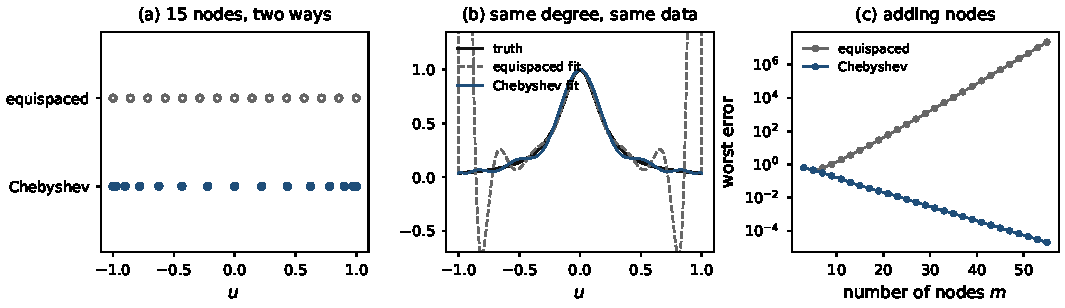
\includegraphics[width=0.94\textwidth]{fig_runge.pdf}
\caption{\small Same function, same polynomial degree, same number of data points. The only
difference is where the points sit. Every curve is computed, not sketched.}
\label{fig:runge}
\end{figure}

\subsection{Why: interpolation amplifies error, by a known factor}

To see what is going on, compare the interpolant with the \emph{best} polynomial of the same
degree, $p^\star$, the one with the smallest worst-case error. Interpolation cannot beat it,
but how much worse can it be?

\begin{prop}[the Lebesgue bound]
\label{prop:lebesgue}
For any continuous $f$ on $[-1,1]$,
\begin{equation}
  \|f-\mathcal{I}_m f\|_\infty \;\le\; \big(1+\Lambda_m\big)\,\|f-p^\star\|_\infty,
  \qquad
  \Lambda_m = \max_{u\in[-1,1]} \sum_{j=1}^{m} \big|\ell_j(u)\big|,
  \label{eq:lebesgue}
\end{equation}
where $\ell_j$ is the Lagrange polynomial equal to $1$ at $u_j$ and $0$ at the other nodes.
\end{prop}

\begin{proof}
A polynomial of degree $m-1$ is its own interpolant, so $\mathcal{I}_m p^\star = p^\star$.
Hence $f - \mathcal{I}_m f = (f-p^\star) - \mathcal{I}_m(f-p^\star)$. The interpolant of any
function $h$ is $\sum_j h(u_j)\ell_j$, so $|\mathcal{I}_m h(u)| \le \|h\|_\infty \sum_j|\ell_j(u)|
\le \Lambda_m\|h\|_\infty$. Apply this with $h = f-p^\star$ and use the triangle inequality.
\end{proof}

\begin{reading}
The right-hand side has two factors with completely different characters.
$\|f-p^\star\|$ is about the \emph{function}: how well polynomials of this degree can do at
all. $\Lambda_m$, the \emph{Lebesgue constant}, is about the \emph{nodes alone} --- it does
not involve $f$. Think of it as an amplifier: it says how much an error in the data can be
magnified on its way to the fitted curve. A good node set keeps the amplifier small.
\end{reading}

\noindent And the two node families have very different amplifiers:
\begin{equation}
  \Lambda_m^{\text{equispaced}} \sim \frac{2^{m}}{e\,m\log m}
  \qquad\text{versus}\qquad
  \Lambda_m^{\text{Chebyshev}} \sim \frac{2}{\pi}\log m .
\end{equation}
Exponential against logarithmic. That is the entire explanation of Figure \ref{fig:runge}:
with equispaced nodes the amplifier grows faster than the best polynomial improves, so
adding nodes loses; with Chebyshev nodes the amplifier barely grows, so the error tracks the
best possible one.

\subsection{The cosine trick behind Chebyshev polynomials}

\begin{idea}
Chebyshev nodes look clustered toward the ends of $[-1,1]$. They are actually \emph{evenly
spaced} --- around a circle. Project evenly spaced points on a semicircle down onto its
diameter and you get exactly this clustering. All the good behaviour comes from that change
of variable, $u = \cos\vartheta$.
\end{idea}

\noindent Define the \emph{Chebyshev polynomial} of degree $k$ by
\begin{equation}
  T_k(\cos\vartheta) = \cos(k\vartheta).
  \label{eq:chebdef}
\end{equation}
That this is a polynomial in $u=\cos\vartheta$ follows from the trigonometric identity
$\cos\big((k{+}1)\vartheta\big) + \cos\big((k{-}1)\vartheta\big) = 2\cos\vartheta\cos(k\vartheta)$,
which in the new variable reads
\begin{equation}
  T_0(u)=1,\qquad T_1(u)=u,\qquad T_{k+1}(u) = 2u\,T_k(u) - T_{k-1}(u).
  \label{eq:recurrence}
\end{equation}
This three-term recurrence is how they are computed in practice: cheap, stable, and needing
nothing more than multiplication. Two properties follow immediately from
\eqref{eq:chebdef}. Every $T_k$ oscillates between $-1$ and $+1$ on the interval, so no
basis function dominates the others; and the points where $T_{m-1}$ reaches $\pm1$, the
\emph{Chebyshev extrema},
\begin{equation}
  u_j = -\cos\!\Big(\frac{\pi(j-1)}{m-1}\Big),\qquad j = 1,\dots,m,
  \label{eq:extrema}
\end{equation}
are evenly spaced in the angle $\vartheta$. Those are the nodes the solver uses.

The extrema have one more property, which matters a great deal in \S\ref{sec:smolyak}: they
are \emph{nested}. With $m = 2^{i-1}+1$ points at ``level'' $i$,
\[
  \{0\}\;\subset\;\{-1,0,1\}\;\subset\;\{-1,-\tfrac{\sqrt2}{2},0,\tfrac{\sqrt2}{2},1\}\;\subset\;\cdots
\]
every point of a coarse level reappears in every finer level. So a solution computed on a
coarse grid is already correct at the points it shares with the next one.

\begin{incode}
\code{chebyshev\_basis\_1d} in \file{state\_grid.py} is the recurrence \eqref{eq:recurrence};
\code{\_level\_points} is \eqref{eq:extrema}; \code{\_new\_points} returns the points a level adds
to the one below, which by nesting are just every other entry.
\end{incode}

\subsection{How fast does it converge? It depends on smoothness}

With good nodes, the error is governed by the best-approximation term in \eqref{eq:lebesgue},
which depends on how smooth $f$ is. Two cases matter here, and the model contains both.

\paragraph{Smooth functions converge geometrically.}

\begin{thm}[analytic functions]
\label{thm:geom}
Suppose $f$ extends to an analytic function on the region bounded by the ellipse in the
complex plane with foci $\pm1$ and semi-axes summing to $\rho>1$, and is bounded there by $M$.
Then interpolation at $m$ Chebyshev extrema satisfies
\begin{equation}
  \|f-\mathcal{I}_m f\|_\infty \;\le\; \frac{4M}{\rho-1}\,\rho^{-(m-1)}.
  \label{eq:geom}
\end{equation}
\end{thm}

\begin{reading}
Every extra node multiplies the error bound by $1/\rho$. So the error falls
\emph{geometrically}, and the rate $\rho$ is set by something you can locate: the largest
such ellipse is the one that just touches $f$'s nearest singularity in the complex plane. A
function whose nearest singularity is far from $[-1,1]$ has a large $\rho$ and is fitted with
few nodes; one whose singularity is close needs many.
\end{reading}

\noindent This is more than a convergence guarantee; it is a \emph{prediction}. Runge's
function has poles at $u=\pm i/5$, only $0.2$ away from the interval, which gives
$\rho = 1.22$: about $11.6$ extra nodes per factor of ten in accuracy. That is the slope of
the Chebyshev line in Figure \ref{fig:runge}(c). We will make the same prediction for this
model's own curved object in \S\ref{sec:refine}, and it will hold there too.

\paragraph{Kinked functions do not.} If $f$ has a corner, like $\max(u,0)$, no ellipse
around the interval avoids a singularity: the theorem gives nothing. The error then falls
only like $1/m$, and worse, it does not fall \emph{uniformly}. Figure \ref{fig:kink}(a,b)
shows the fit of $\max(u,0)$ at three resolutions. Near the corner the polynomial overshoots,
and adding nodes makes the overshoot \emph{narrower but not smaller}: it migrates toward the
corner and keeps its height. This is the \emph{Gibbs phenomenon}.

\begin{figure}[t]
\centering
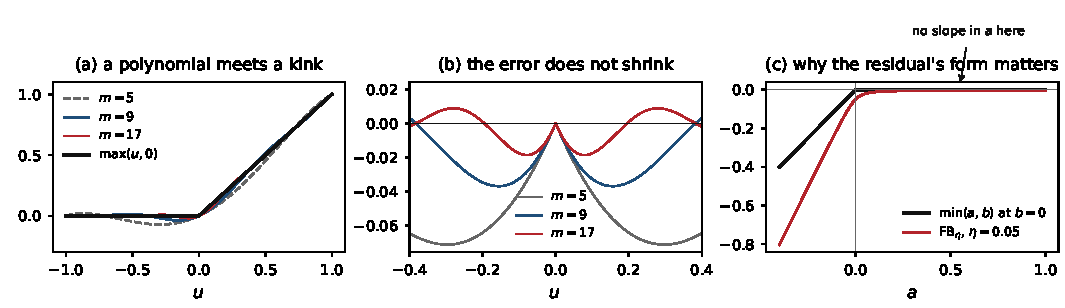
\includegraphics[width=0.94\textwidth]{fig_kink.pdf}
\caption{\small A polynomial meets a kink. (a) Fits of $\max(u,0)$ come out positive where the
truth is exactly zero. (b) Refinement narrows the error but does not shrink it. (c) A
preview of \S\ref{sec:kink}: two ways of writing ``one of these is zero'' differ in whether
they carry any slope.}
\label{fig:kink}
\end{figure}

\noindent The lesson is worth stating plainly, because it governs a real limitation in
\S\ref{sec:kink}: \emph{more resolution cures smooth error quickly and kinked error hardly at
all.} When a model's answer depends on behaviour right at a kink, the fix has to come from
somewhere other than more nodes.

\subsection{Why we interpolate instead of fitting by least squares}

An alternative is to sample more points than coefficients and fit by least squares, which is
more robust to noisy data. The solver deliberately does not do this. With exactly as many
nodes as basis functions, the coefficients solve a \emph{square} linear system,
\begin{equation}
  \Phi\,\bm c = \bm y,\qquad \Phi_{ij} = \phi_j(u_i),
  \label{eq:square}
\end{equation}
and the fitted function passes \emph{exactly} through every data point. Part II will make the
policy's values \emph{at the nodes} the unknowns of the whole problem, and the solver will
read tomorrow's decisions off the fitted function. If the fitted function did not reproduce
its own nodes, ``the value of the policy at a node'' would mean two different things at once,
and the system would be inconsistent with itself. So exactness at the nodes is a structural
requirement, not a convenience. A bonus: $\Phi$ depends only on the grid, so it is factored
once and every refit afterwards costs only a triangular solve.

\begin{lever}{the number of nodes $m$ (one dimension)}
\leverrow{Controls}{The polynomial degree, $m-1$, and the cost of every function evaluation.}
\leverrow{Push to 1}{A constant. Every state looks the same; the rule cannot respond to
anything.}
\leverrow{Push to $\infty$}{For smooth $f$ the error vanishes geometrically, at the rate set
by the nearest complex singularity \eqref{eq:geom}. For kinked $f$ it barely moves, since the
Gibbs overshoot only narrows. In many dimensions the cost of large $m$ is ruinous, which is
the subject of the next section.}
\leverrow{Here}{Chosen per dimension: two levels in most dimensions, and a dense factor of $5$
(confirmed by a run at $9$) in the one dimension that carries real curvature
(\S\ref{sec:refine}).}
\end{lever}

%======================================================================
\section{Many variables: the curse, and Smolyak's way around it}
\label{sec:smolyak}

\subsection{The curse, concretely}

The obvious way to go from one dimension to many is to take every combination. With $m$
nodes per dimension in $d$ dimensions, the \emph{tensor-product grid} has $m^d$ points and
the matching basis contains every product $T_{k_1}(u_1)\,T_{k_2}(u_2)\cdots T_{k_d}(u_d)$.
It inherits all the one-dimensional accuracy. It also inherits an exponential bill. This model
has $d=12$, so even a modest $m=5$ gives
\[
  5^{12} \approx 2.4\times10^{8}\ \text{points},
\]
and at each point the solver must evaluate the entire economy, including an expectation over
tomorrow. That is not slow; it is impossible, by roughly eight orders of magnitude. Any method
that works must avoid most of these points.

\subsection{The key observation: you rarely need every interaction}

\begin{idea}
Look at what the tensor grid is paying for. A basis function like
$T_4(u_1)\,T_4(u_2)\,T_4(u_3)$ describes a degree-4 wiggle in three variables
\emph{simultaneously}. For a smooth function such terms are tiny: if each variable separately
needs only a little curvature, their high-order \emph{joint} curvature is smaller still. So
keep high degree in one variable at a time, keep low-order interactions between variables,
and drop the high-order joint terms. That is the whole of Smolyak's idea; the rest is
bookkeeping to do it consistently.
\end{idea}

\subsection{Building the grid from differences, one step at a time}

The bookkeeping is easiest to see by splitting interpolation into increments.

\paragraph{Step 1: levels in one dimension.} Let $\mathcal{I}^{(i)}$ be one-dimensional
interpolation on the level-$i$ node set from \S\ref{sec:1d} ($1$, $3$, $5$, $9,\dots$ nodes),
and set $\mathcal{I}^{(0)}\equiv 0$.

\paragraph{Step 2: what each level adds.} Define the \emph{difference operator}
\begin{equation}
  \Delta^{(i)} \;=\; \mathcal{I}^{(i)} - \mathcal{I}^{(i-1)} .
\end{equation}
$\Delta^{(i)}$ is ``the correction level $i$ makes to level $i-1$''. For a smooth function
these corrections shrink quickly as $i$ grows --- that is just geometric convergence again.

\paragraph{Step 3: telescoping.} Summing the corrections recovers the interpolant,
$\mathcal{I}^{(L)} = \Delta^{(1)} + \Delta^{(2)} + \dots + \Delta^{(L)}$.

\paragraph{Step 4: two dimensions.} The full tensor interpolant at level $L$ in both
directions is then a double sum,
\begin{equation}
  \mathcal{I}^{(L)}\otimes\mathcal{I}^{(L)}
  = \sum_{i_1=1}^{L}\sum_{i_2=1}^{L}\Delta^{(i_1)}\otimes\Delta^{(i_2)},
\end{equation}
one term for every cell of an $L\times L$ square of level pairs. The term in cell
$(i_1,i_2)$ is a correction in $u_1$ \emph{times} a correction in $u_2$; when both levels are
high it is the product of two small things.

\paragraph{Step 5: keep only a triangle.} Smolyak's operator keeps the cells below a
diagonal:
\begin{equation}
  \boxed{\;\mathcal{A}_{\mu} \;=\; \sum_{\bm i\,:\;\sum_j (i_j-1)\,\le\,\mu}
  \Delta^{(i_1)}\otimes\Delta^{(i_2)}\otimes\cdots\otimes\Delta^{(i_d)}\;}
  \label{eq:smolyak}
\end{equation}

\begin{reading}
Each dimension's level $i_j$ ``costs'' $i_j-1$, and the total spending across dimensions may
not exceed the \emph{budget} $\mu$. You may spend the whole budget on one dimension (high
resolution there, the base level elsewhere) or split it (moderate resolution in several,
together). What you may not do is spend a lot everywhere at once. Figure
\ref{fig:smolyak}(a) shows the triangle of kept cells for $\mu=2$ in two dimensions;
panels (b) and (c) show the resulting grids.
\end{reading}

\begin{figure}[t]
\centering
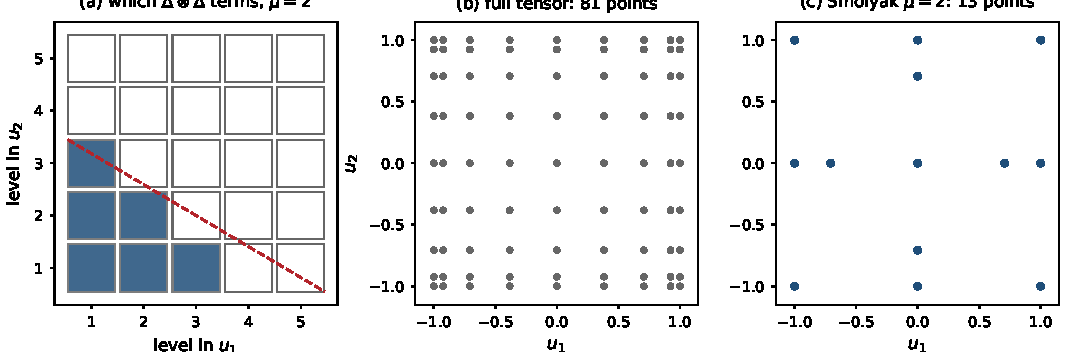
\includegraphics[width=0.94\textwidth]{fig_smolyak.pdf}
\caption{\small (a) The Smolyak budget as a picture: each cell is one
$\Delta^{(i_1)}\otimes\Delta^{(i_2)}$ term, and only the shaded triangle is kept. (b) The full
tensor grid at the same resolution. (c) The Smolyak grid: the axes keep their resolution, and
the high-order corners are dropped. Drawn by the solver's own grid constructor.}
\label{fig:smolyak}
\end{figure}

\paragraph{Step 6: points.} Because the node sets are nested, each kept cell contributes only
the points \emph{new} at its levels, and the grid is the union of those small products. With
budget $\mu=1$ the only admissible level vectors are ``every dimension at level 1'' (one
point, the centre) and ``one dimension at level 2'' (two new points each), so
\begin{equation}
  |\text{grid}| = 1 + 2d \qquad (\mu = 1).
\end{equation}
At $d=12$ that is $25$ points; at $\mu=2$ it is $313$. In general the count grows like
$d^{\mu}$: \emph{polynomially} in the dimension, against the tensor grid's exponential.
That single fact is what makes a twelve-dimensional global solution possible at all.

\subsection{What the budget buys, and what it does not}
\label{sec:exactness}

The budget does not just set the number of points; it sets exactly which functions the fit can
represent.

\begin{prop}[what $\mu=1$ can represent]
\label{prop:span}
At budget $\mu=1$ the fitted functions are exactly the combinations of
\[
  1,\qquad T_1(u_j) = u_j,\qquad T_2(u_j) = 2u_j^2-1,\qquad j=1,\dots,d:
\]
a constant, a slope in each variable, and a curvature in each variable \emph{separately}.
There are no cross terms $u_ju_k$ at all. At $\mu=2$ all pairwise products $u_ju_k$ are
added.
\end{prop}

\noindent This is easy to state and easy to forget, so here is a direct check on the solver's
own grid (twelve dimensions, budget $\mu=1$, refined in the risk dimension as described next).
Fitting $1 + 0.3u_1 - 0.2u_4 + u_9^2 + 0.5\,u_1u_9$, where $u_9$ is the risk state,
reproduces it at $500$ random points to $7\times10^{-16}$ --- machine precision. Fitting
$u_1u_4$, a cross term between two ordinary dimensions, gets it wrong by $0.96$: the fit has
no way to express it and returns something close to zero. \emph{At $\mu=1$ a missing
interaction is not approximated badly; it is not there.} Choosing $\mu$ is therefore a
modelling decision: you are asserting which interactions the economics does not need.

\begin{lever}{the Smolyak budget $\mu$}
\leverrow{Controls}{Which interactions between state variables the rule can express, and the
grid size, which grows like $d^{\mu}$.}
\leverrow{Push to 0}{One point. Every state is treated as the steady state.}
\leverrow{Push up}{Every interaction becomes representable and the grid approaches the full
tensor product; at $d=12$ the cost explodes long before the accuracy needs it.}
\leverrow{Here}{$\mu=1$: no cross terms between ordinary states. The one interaction the
economics clearly needs, between the risk state and everything else, is bought separately by
the refinement below, much more cheaply than by raising $\mu$.}
\end{lever}

\subsection{Making the system square: new points, new degrees}

Written as \eqref{eq:smolyak}, the Smolyak interpolant is a signed sum of many tensor
interpolants, which is awkward to compute with. The solver uses an equivalent construction
that keeps the square system \eqref{eq:square}. Pair each level's \emph{new points} with an
equally large set of \emph{new degrees}: degree $0$ at level 1, degrees $\{1,2\}$ at level 2,
degrees $\{3,4\}$ at level 3, $\{5,\dots,8\}$ at level 4, and so on. Running the same budget
over degrees instead of points produces exactly as many basis functions as nodes. The matrix
$\Phi$ is square, the fit passes through every node, and \S\ref{sec:1d}'s argument for
exactness carries over unchanged.

\subsection{Spending resolution where the curvature is}
\label{sec:refine}

\begin{idea}
This model has one strongly curved object: the default probability $p^d(s) =
1/(1+e^{-s})$, a logistic in the risk factor $s$. Almost everything else is close to linear.
Raising $\mu$ to buy curvature in $s$ would also buy it in eleven dimensions that do not need
it. Instead, make the grid dense in $s$ alone.
\end{idea}

\noindent The construction is a product of two interpolation operators,
\begin{equation}
  \mathcal{A} \;=\; \underbrace{\mathcal{A}_{\mu}^{(\text{all but } s)}}_{\text{sparse, 11 dims}}
  \;\otimes\; \underbrace{\mathcal{I}^{m}_{(s)}}_{\text{dense, } m \text{ nodes in } s} ,
  \label{eq:refine}
\end{equation}
with $(1+2\cdot 11)\times m = 23m$ points at $\mu=1$: $69$, $115$ and $207$ for $m=3,5,9$.
Two things make this the right tool. Both factors are square interpolants, so the product is
square and exact at its nodes. And because it is a full product, every sparse basis function
is multiplied by every power of $s$: the cross term $u_1u_9$ from \S\ref{sec:exactness} is
present for exactly this reason.

How many nodes in $s$? Theorem \ref{thm:geom} answers \emph{before} running anything. The
logistic's nearest singularity is the pole at $s = i\pi$. Mapped into the solver's unit
interval it sits at $u = 1.76 + 0.80i$, giving $\rho = 3.71$. The prediction is that each
extra node in $s$ divides the error by about $3.7$, or roughly one factor of ten for every
$1.8$ nodes. Figure \ref{fig:refine} shows the test on the solver's actual risk box: from
$3$ to $13$ nodes the error falls by a factor of $3.4\times10^5$, against a predicted
$\rho^{10} = 4.9\times10^5$.

\begin{figure}[t]
\centering
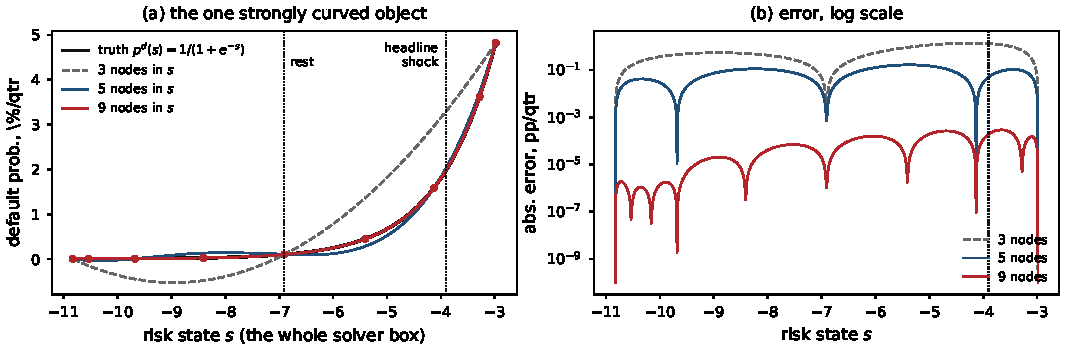
\includegraphics[width=0.94\textwidth]{fig_refine.pdf}
\caption{\small Fitting the logistic $p^d(s)$ across the solver's own risk box. With three
nodes (a quadratic) the fit reads $3.30\%$ at the headline shock, where the truth is $1.98\%$,
and goes \emph{negative} near $s=-9$: a probability below zero. Five nodes read $2.03\%$; nine
read $1.980\%$. The dots are the nodes; all three fits share the rest point as a node.}
\label{fig:refine}
\end{figure}

\noindent Notice what the three-node fit does. It reads the headline shock's $1.98\%$ default
probability as $3.30\%$, and it makes a probability \emph{negative}. A rule fitted that
coarsely would price risk that is not there. This is the concrete content of the
refinement: not a smaller error bar, but the difference between pricing the shock and
mispricing it by two thirds.

\begin{lever}{the dense factor in the risk dimension, $m_s$}
\leverrow{Controls}{The degree in $s$ ($m_s-1$) and its full interaction with every other
state; the grid size $23m_s$.}
\leverrow{Push to 1}{The rule ignores risk entirely.}
\leverrow{Push to 3}{A quadratic in $s$: the headline shock is mispriced by two thirds and
default probabilities can come out negative (Figure \ref{fig:refine}).}
\leverrow{Push up}{Error falls by about $3.7$ per node, as predicted, but the solver's cost
grows with the \emph{square} of the grid size (\S\ref{sec:newton}): $9$ nodes ($207$ points)
costs about $(207/115)^2\approx3.2$ times as much as $5$.}
\leverrow{Here}{$5$, confirmed by a run at $9$: the headline output response moved
$1.6$--$3.4\%$ of itself, and every other reported number moved in the third digit.}
\end{lever}

\begin{incode}
\code{SmolyakGrid} in \file{state\_grid.py} builds the grid; \code{\_multi\_indices} enumerates
the budget's level vectors, \code{\_new\_degrees} pairs degrees with points, and
\code{refine=(dim, m)} applies \eqref{eq:refine} via \code{\_tensor\_refine}. The shipped
setting is \code{S\_REFINE = 5} (the number of dense nodes in $s$) in \file{run.py}.
\end{incode}

%======================================================================
\section{The box: where the approximation lives}
\label{sec:box}

\begin{idea}
A global method is global only on a region, a box of states. Outside the box the polynomial is
\emph{extrapolating}, and polynomial extrapolation is wildly unreliable. So the box must
contain everywhere the economy actually goes. But every bit of width spent on states the
economy never visits is resolution taken away from states it does.
\end{idea}

\subsection{Mapping the box to the unit cube}

Each state $S_j$ has bounds $[\underline S_j,\overline S_j]$, and the grid of
\S\ref{sec:smolyak}, built on $[-1,1]$, is stretched onto it:
\begin{equation}
  u_j = 2\,\frac{S_j-\underline S_j}{\overline S_j-\underline S_j} - 1 .
\end{equation}
The affine map changes nothing in the theory, with one consequence worth noting:
\emph{widening} a dimension spreads the same nodes over more ground, so for a fixed node count
a wider box is a coarser fit.

\subsection{Measure width in standard deviations, not units}

For the stochastic state $s$, which follows $s' = (1-\rho_s)\bar s + \rho_s s + \sigma_s\varepsilon$,
the natural unit is its unconditional standard deviation $\sigma_s/\sqrt{1-\rho_s^2}$. The
box is set to
\begin{equation}
  s \in \Big[\,\bar s - \kappa\,\tfrac{\sigma_s}{\sqrt{1-\rho_s^2}},\;
  \bar s + \kappa\,\tfrac{\sigma_s}{\sqrt{1-\rho_s^2}}\,\Big],
\end{equation}
so that the coverage $\kappa$ is the lever, not an absolute width. With $\sigma_s = 0.4455$,
$\rho_s = 0.95$ and $\kappa = 2.75$, the half-width is $3.92$ and the box runs from a $0.002\%$
to a $4.82\%$ quarterly default probability. The headline shock sits $77\%$ of the way to the
edge.

Why insist on standard-deviation units? Because an absolute width silently changes coverage
whenever $\sigma_s$ is recalibrated. This is not a hypothetical. In this model's history, a box
sized in absolute units turned out to be only $1.4$ to $2.3$ \emph{conditional} standard
deviations wide. Simulated states that left it were projected back to its edge, and that
projection mean-reverted $s$ harder than the AR(1) itself did: the \emph{effective}
persistence fell from $0.95$ to $0.80$. Since the long bond's repricing comes from persistent
risk, about $62\%$ of the paper's mechanism disappeared --- with no error message. A box is part
of the model.

\begin{lever}{box coverage $\kappa$ (and the bands on the other states)}
\leverrow{Controls}{Which states the rule is accurate on, and how finely.}
\leverrow{Push small}{The economy leaves the box. Either the rule extrapolates (unreliable) or
states are clipped back in, which secretly changes the model's dynamics --- here, the
persistence of risk.}
\leverrow{Push large}{The same nodes spread over states the economy never visits; accuracy
where it does live degrades, and corners of the box may be states where the model has no
solution at all.}
\leverrow{Here}{$\kappa = 2.75$, chosen so the headline shock ($2.11$ standard deviations) sits
well inside rather than at the edge. The capital, deposit and bond bands are a few percent of
their steady-state values; \S\ref{sec:accuracy} reports how often the simulated economy
leaves them.}
\end{lever}

\subsection{A surprise: a stable economy whose box cannot be stable}

Ideally the box is \emph{invariant}: from any state inside, the economy stays inside next
period. Near the steady state the law of motion is approximately linear, $\st'-\bar\st
\approx J(\st-\bar\st)$. When is an axis-aligned box with half-widths $\bm b$ invariant? The
worst case pushes every coordinate to its edge with signs chosen to maximise the image, which
gives the condition
\begin{equation}
  |J|\,\bm b \;\le\; \bm b \quad\text{componentwise},
  \label{eq:invariance}
\end{equation}
where $|J|$ takes absolute values entry by entry. By the Perron--Frobenius theorem a positive
$\bm b$ solving \eqref{eq:invariance} exists only if the spectral radius $\rho(|J|) \le 1$.

The surprise is that $\rho(|J|)$ is not $\rho(J)$. For the block of the two banks' deposit
bills, the solver measured
\begin{equation}
  J = \begin{pmatrix} 1.076 & -0.310 \\ 2.016 & -1.252 \end{pmatrix}:
  \qquad \text{eigenvalues } 0.766,\ -0.942,
  \qquad \rho(|J|) = 1.96 .
\end{equation}
The dynamics are stable, since both eigenvalues are inside the unit circle. And yet no
axis-aligned box around the steady state is invariant, at any size. The reason is that $J$ is
\emph{non-normal}: its singular values are $2.61$ and $0.28$, so it stretches hard in one
diagonal direction while shrinking in another. Over several periods the shrinking wins, but in
a single step a corner of the box is pushed outside it.

\paragraph{The fix in theory, and why it was turned off.} Draw the box in the eigenvector
coordinates $\bm z = V^{-1}(\st-\bar\st)$, where $J$ is diagonal and every box is invariant.
The solver supports this. It also measured that it is worse: a box that is rectangular in
eigen-coordinates is a parallelogram in the original ones, and its corners reach combinations
of the two deposit bills at which the economy has no solution. The rotation ships switched
off. This is a pattern worth expecting: \emph{the correct geometric argument tells you what to
try; only measurement tells you what to keep.}

\paragraph{A shear that is kept.} For the central bank's bond book, the opposite happened. A
bond purchase moves the bank's holding and the central bank's holding one-for-one and creates a
claim proportional to both. On the natural axes, most corners of the box are states no
purchase can produce, and fitting through them made the bond price respond to purchases
non-monotonically. Re-drawing the box on the directions purchases actually move along (a
\emph{shear}, with determinant one) removed the problem. Because those two states are zero at
the steady state, the old ten-state grid survives exactly as the slice where they vanish, so
switching the policy off reproduces the old solution to solver precision (measured:
$5.5\times10^{-10}$).

\begin{incode}
\code{build\_state\_box} in \file{state\_grid.py} sets every band, the $s$ coverage
(\code{S\_COVER\_SD}, the coverage $\kappa$) and the shear; the shared bands for both experiments
are \code{BOX\_KW} in \file{recursive\_experiment.py}. \code{p\_block\_rotation} in
\file{recursive\_main.py} measures $J$; the rotation switch is \code{ROTATE\_P} in \file{run.py}.
\end{incode}

%======================================================================
\part*{Part II \quad Finding the coefficients}
\addcontentsline{toc}{section}{\textbf{Part II\quad Finding the coefficients}}
%======================================================================
\section{Two ways to solve a functional equation}
\label{sec:paradigms}

\begin{idea}
Part I chose the family of functions and the points at which to check the equation. What
remains is a large system of nonlinear equations. There are two strategies. The first
\emph{iterates}: guess tomorrow's behaviour, work out today's best response, adopt it as the
new guess for tomorrow, and repeat until nothing changes. The second \emph{solves}: treat the
whole rule as unknown at once and hand every equation at every node to a single root-finder.
The first is the textbook default. In this model it fails in a way that is easy to miss, and
the reason is worth understanding.
\end{idea}

\subsection{Time iteration}

Fix a guess $\hat g^{(k)}$. At each node $\st_i$, treat $\hat g^{(k)}$ as the rule people
expect to follow tomorrow, and solve the period's equilibrium conditions for today's
decisions:
\begin{equation}
  x_i^{\text{new}}\ \text{ solves }\ \mathcal F\Big(\st_i,\,d,\,x_i^{\text{new}},\,
  \E\big[\hat g^{(k)}(\st',d')\big]\Big) = \bm 0 .
\end{equation}
Fit a new rule through the $x_i^{\text{new}}$, call that map $\mathcal T$, and update with
damping $\omega\in(0,1]$:
\begin{equation}
  \hat g^{(k+1)} \;=\; (1-\omega)\,\hat g^{(k)} + \omega\,\mathcal{T}\big[\hat g^{(k)}\big].
  \label{eq:ti}
\end{equation}
The attractions are real. Each node's problem is small ($14$ unknowns, not thousands); nodes
are independent of one another; and if $\mathcal T$ is a contraction the iteration converges
from almost any start.

\subsection{The trap is in the contraction rate}

Suppose $\mathcal T$ contracts at rate $\rho_{\mathcal T}$: each application shrinks the
distance to the answer by that factor. Damping slows it to
\begin{equation}
  \rho \;=\; 1-\omega\,(1-\rho_{\mathcal T})
\end{equation}
per sweep. Everything then hinges on how close $\rho$ is to one, and in this model it is very
close. The slowest-moving part of the rule is the bank's \emph{franchise value} $\alpha$, the
value to a banker of an extra unit of net worth. It satisfies a recursion of the form
\begin{equation}
  \alpha \;=\; \frac{\E[\Omega']\,R}{1-\mu},\qquad
  \Omega' \;=\; \beta\big[f + (1-f)\,\alpha'\big],
  \label{eq:franchise}
\end{equation}
where $f$ is the share of bankers who exit each period, $R$ the gross deposit rate and $\mu$
the shadow value of the borrowing limit. Differentiate today's $\alpha$ with respect to
tomorrow's $\alpha'$:
\begin{equation}
  \frac{\partial\alpha}{\partial\alpha'} \;=\; \frac{\beta(1-f)R}{1-\mu}
  \;\approx\; \frac{1-f}{1-\mu},
  \label{eq:slope}
\end{equation}
where the approximation uses $\beta R\approx1$, which holds by construction here because the
banker's discount factor is set to $1/R$ in the steady state.

\begin{reading}
Two things can be read straight off \eqref{eq:slope}. First, at the calibration
($f=0.08$, $\mu\approx0.012$) the slope is $0.93$. Each sweep of time iteration therefore
removes only $7\%$ of the remaining error in $\alpha$, and with damping $\omega=0.25$ only
$1.7\%$. That is $133$ sweeps for every factor of ten; the rate measured on the full model
during development was slower still, $0.990$ per sweep, or $229$ sweeps per factor of ten.
Second, the slope exceeds one --- the recursion becomes \emph{explosive} --- exactly when
$\mu > f$. At this calibration that threshold is $\mu = 0.080$, which the deep corners of the
default regime can reach. That is why the code caps $\alpha$ (\S\ref{sec:reference}).
\end{reading}

\noindent A slow contraction is merely slow. What makes it dangerous is how one decides to
stop.

\begin{prop}[the stopping-rule trap]
\label{prop:stall}
If the iteration contracts at rate $\rho<1$ and is stopped when successive iterates differ by
less than $\tau$, the remaining distance to the answer can be as large as
\begin{equation}
  \|\hat g^{(k)} - g\| \;\le\; \frac{\tau}{1-\rho}.
\end{equation}
\end{prop}

\begin{proof}
The remaining distance is at most the sum of all future steps, each a factor $\rho$ smaller
than the last:
\[
  \|\hat g^{(k)}-g\| \;\le\; \sum_{j\ge0}\|\hat g^{(k+j+1)}-\hat g^{(k+j)}\|
  \;\le\; \tau\sum_{j\ge0}\rho^{j} \;=\; \frac{\tau}{1-\rho}. \qedhere
\]
\end{proof}

\noindent At $\rho = 0.99$ a tolerance of $10^{-6}$ admits an error of $10^{-4}$, a hundred
times what the stopping rule appears to promise. The symptom in practice was striking and
worth recognising: runs reported a worst equation residual of $10^{-14}$ \emph{and}
``rule-change tolerance not reached'' at the same time. Every node was solving its equations
perfectly --- against a picture of tomorrow that was still moving. The residual, the obvious
thing to monitor, said nothing about the error.

\begin{lever}{the damping weight $\omega$ in time iteration}
\leverrow{Controls}{How far each sweep moves toward the new best response.}
\leverrow{Push to 0}{Nothing moves. Perfectly stable and perfectly useless.}
\leverrow{Push to 1}{The fastest contraction ($0.93$ per sweep here), but an undamped
iteration can overshoot and oscillate wherever $\mathcal T$ is steep, for instance near the
switch in $\mu$, and the explosive region $\mu>f$ is never far away in the default corners.}
\leverrow{Here}{$0.5$, and time iteration is used only for a short warm start ($12$ sweeps,
$20$ on refined grids). It is never asked to converge; that job belongs to Newton.}
\end{lever}

\subsection{Simultaneous collocation: make the node values the unknowns}

The alternative abandons the operator. Collect the value of every rule at every node, in each
of the two default regimes, into one long vector,
\begin{equation}
  \pol = \Big(\,\hat x_k(\st_i,d)\,\Big)_{k=1..20,\;d=0,1,\;i=1..115}\;\in\;\R^{4600},
\end{equation}
and define a single map $F:\R^{4600}\to\R^{4600}$ that does three things in sequence:
\begin{enumerate}
\item fit Chebyshev coefficients to the values in $\pol$ (one triangular solve per rule);
\item at every node and regime, evaluate the period's equilibrium conditions, using
\emph{that} fitted rule to form tomorrow's expectations;
\item stack the resulting residuals into one vector.
\end{enumerate}
Then find $\pol$ with $F(\pol)=\bm 0$ by Newton's method. Notice what has disappeared: there is
no inner root-finding at each node, and no frozen picture of tomorrow. Tomorrow is always read
off the current guess, so whenever $F(\pol)=\bm0$ the rule is consistent with itself by
construction. There is no contraction rate for error to hide in, because the solver drives
the residual itself to zero.

\subsection{The self-reference trick: identity residuals}

One subtlety makes this work. Six of the stored rules --- the two franchise values $\alpha$,
the two consumption levels, and the two working-capital interest rates --- are not chosen by
any first-order condition. In time iteration they were \emph{read off} recursions like
\eqref{eq:franchise}, given the frozen rule for tomorrow. In simultaneous collocation they
must be unknowns too, or the system is not square. What equation pins them? Their own
definition: the guessed value must equal the value the recursion implies,
\begin{equation}
  r_k \;=\; \log\frac{\text{guess}_k}{\text{implied}_k} \;=\; 0 .
  \label{eq:identity}
\end{equation}

\begin{reading}
The logarithm makes the residual a percentage gap, so a franchise value near $1.2$ and an
interest rate near $0.003$ are measured on the same scale. And here the square system of
\S\ref{sec:1d} pays off. When the period map asks for $\alpha$ at the current node, the fitted
function returns \emph{exactly} the guessed value, because a square interpolant reproduces its
own nodes. So \eqref{eq:identity} carries no interpolation error at all: it is a clean
self-consistency condition. Counting gives $14$ economic residuals plus these $6$, which is
$20$ per node and regime, matching the $20$ stored rules.
\end{reading}

\begin{incode}
\file{collocation.py} is the solver. \code{make\_residual} builds $F$;
\code{pack}/\code{unpack} fix the order of the $4600$ unknowns; \code{\_point\_block} appends
\eqref{eq:identity}. The per-node economics is \code{point\_residuals} in \file{point\_map.py},
the same function time iteration calls --- only the caller changes. The warm start is
\code{time\_iteration} in \file{recursive\_main.py}.
\end{incode}

%======================================================================
\section{Newton's method on 4600 unknowns}
\label{sec:newton}

\begin{idea}
Newton's method replaces the nonlinear problem with its best linear approximation at the
current guess, solves that exactly, and jumps there. Near a root this is spectacularly fast:
the number of correct digits roughly doubles each step. Far from a root it can do anything at
all. Most of the engineering around Newton is about the second sentence.
\end{idea}

\subsection{The step}

At the current guess $\pol^{(k)}$, approximate $F$ by its tangent plane,
$F(\pol) \approx F(\pol^{(k)}) + J\,(\pol-\pol^{(k)})$, where $J$ is the Jacobian matrix of
partial derivatives. Setting the approximation to zero and taking a damped step gives
\begin{equation}
  \pol^{(k+1)} \;=\; \pol^{(k)} - c\,J^{-1}F(\pol^{(k)}),\qquad c\in(0,1].
  \label{eq:newton}
\end{equation}
With $4600$ unknowns, $J$ is $4600\times4600$: about twenty-one million entries.

\subsection{Getting the Jacobian by finite differences}

$F$ contains interpolation, quadrature, fractional powers and smoothed maximum functions; an
analytic $J$ is out of reach. Instead, nudge one unknown at a time:
\begin{equation}
  J_{:,j} \;\approx\; \frac{F(\pol+\varepsilon\bm e_j) - F(\pol)}{\varepsilon},
  \label{eq:fd}
\end{equation}
where $\bm e_j$ is the $j$-th unit vector. How big should the nudge $\varepsilon$ be? Two errors
pull in opposite directions. By Taylor's theorem, the quotient misses the true derivative by
about $\tfrac12\varepsilon M$, where $M$ bounds the second derivative: \emph{small} $\varepsilon$
reduces this. But each evaluation of $F$ carries some noise $\delta$, and dividing a difference
of noisy numbers by $\varepsilon$ magnifies the noise to about $2\delta/\varepsilon$:
\emph{large} $\varepsilon$ reduces this. Minimising the sum,
\begin{equation}
  \text{error}(\varepsilon) \approx \tfrac12\varepsilon M + \frac{2\delta}{\varepsilon}
  \quad\Longrightarrow\quad
  \varepsilon^\star = 2\sqrt{\delta/M}.
  \label{eq:fdstep}
\end{equation}

\begin{reading}
Both ingredients are specific to the function being differentiated. \emph{The noise $\delta$}:
if it were only machine rounding, $\delta\approx10^{-16}$ and $\varepsilon^\star\approx10^{-8}$,
the familiar textbook value. But this $F$ has a measured arithmetic floor near $10^{-10}$ ---
its Euler equations take differences of order-one expectations that nearly cancel --- and with
that $\delta$ the optimum moves up to $\varepsilon^\star\approx2\times10^{-5}$. \emph{The
curvature $M$}: it is not one number. On the smooth parts of $F$ it is of order one. But on a
kink that has been smoothed over a width $\eta$ (\S\ref{sec:kink}), the slope turns over a
distance $\eta$, so $M\approx1/\eta$, and the truncation term becomes
\begin{equation*}
  \tfrac12\,\varepsilon M \;\approx\; \frac{\varepsilon}{2\eta}:
\end{equation*}
a \emph{relative} error in the computed slope, which is small only if $\varepsilon\ll\eta$.
That is the precise meaning of ``the nudge must not jump across the bend.''
\end{reading}

\noindent This formula is predictive. The solver once ran with smoothing $\eta=10^{-5}$ against
its step $\varepsilon=10^{-6}$; the formula gives $\varepsilon/2\eta = 5\%$, and the measured
Jacobian near the affected switch was indeed ``off by several percent,'' enough to turn
Newton's quadratic convergence linear. Raising the smoothing to $10^{-4}$ cut the predicted error
to $0.5\%$ and restored it. The shipped $\varepsilon = 10^{-6}$ is therefore a compromise between
two optima --- about $2\times10^{-5}$ on the smooth parts and $2\sqrt{\delta\eta}\approx2\times10^{-7}$
on the smoothed kinks --- and errs toward the kinks, where a bad slope costs most.

\begin{lever}{the finite-difference step $\varepsilon$}
\leverrow{Controls}{The accuracy of the Jacobian, hence how fast Newton converges.}
\leverrow{Push small}{The $2\delta/\varepsilon$ term takes over: the columns become amplified
rounding noise and the Newton direction is garbage.}
\leverrow{Push large}{Truncation error grows, and on a smoothed kink it is a relative slope
error of $\varepsilon/2\eta$. At $\varepsilon=\eta/10$ that is $5\%$: measured here as a Jacobian
``off by several percent'' and Newton converging only linearly.}
\leverrow{Here}{$10^{-6}$: between the smooth-part optimum ($2\times10^{-5}$) and the kink optimum
($2\times10^{-7}$), and two decades below the narrowest smoothing, so the worst relative slope
error is $0.5\%$ (Figure \ref{fig:window}).}
\end{lever}

\subsection{What Newton promises, and what it does not}

\begin{thm}[local quadratic convergence]
\label{thm:newton}
Suppose $F$ is continuously differentiable near a root $\pol^\star$, $J(\pol^\star)$ is
invertible, and $J$ changes no faster than a Lipschitz constant $L$ allows. Then there is a
neighbourhood of $\pol^\star$ from which the undamped iteration converges, and
\begin{equation}
  \|\pol^{(k+1)}-\pol^\star\| \;\le\; \tfrac12 L\,\|J(\pol^\star)^{-1}\|\;
  \|\pol^{(k)}-\pol^\star\|^2 .
  \label{eq:quadratic}
\end{equation}
\end{thm}

\begin{reading}
The error on the right is \emph{squared}. Once the error is small, $10^{-3}$ becomes about
$10^{-6}$, then $10^{-12}$: the number of correct digits roughly doubles each step. The solver's
main solve --- all $4600$ unknowns on the refined grid, in the current run --- shows exactly that:
the worst residual went $8.5\times10^{-3}\to2.6\times10^{-5}\to3.3\times10^{-9}$ in three full steps,
from two correct digits to about four and a half to eight and a half, and then stopped because it had
reached the arithmetic floor. Compare time iteration's $229$ sweeps per factor of ten.
\end{reading}

\noindent Read the theorem's hypotheses, though, because two things it does \emph{not} say
shape everything that follows.

\paragraph{It is local.} The guarantee holds only inside a neighbourhood whose size depends on
$L$ and $\|J^{-1}\|$, neither of which you know. Start outside it and Newton may diverge,
cycle, or step to a point where $F$ cannot even be evaluated. \S\ref{sec:homotopy} is entirely
about starting inside.

\paragraph{It does not say which root.} Newton finds \emph{a} root. With a switching constraint
there are genuinely different nearby solutions --- one where the constraint binds and one where
it does not --- and a step can slip from one to the other. This happened here. Re-solving the
equations at each simulated state, starting from the fitted rule, slipped onto the slack
solution in $49$ of $60$ periods: the multiplier walked from $0.103$ to zero and the output
response changed sign, from $-0.004\%$ to $+2.5\%$. The remedy, in \S\ref{sec:reading}, is to
\emph{read} the solved rule rather than re-solve.

\subsection{Globalisation, and knowing when you are done}

Two practical additions turn the local method into a usable one.

\paragraph{A line search.} Measure progress by $\varphi(\pol)=\tfrac12\|F(\pol)\|_2^2$. Try the
full step; if $\varphi$ does not fall, halve the step, and repeat. Since the Newton direction
always points downhill for $\varphi$ (its directional derivative is $-\|F\|^2<0$), a small enough
step always helps --- unless $F$ is already at its noise floor.

The current run's first stage shows the two phases this produces. For four steps the line search cut
the step to $\tfrac14$, $\tfrac12$, $\tfrac12$ and $\tfrac18$ and progress was slow: the guess was
outside the region where the linear model is trustworthy. (The worst single residual even
\emph{rose}, from $4.5\times10^{-3}$ to $5.3\times10^{-3}$, while $\varphi$ fell; the line search watches
the sum of squares, not the largest entry.) Then full steps took over, landing at $1.7\times10^{-5}$, $6.1\times10^{-7}$ and
$1.3\times10^{-10}$ in turn. Slow and careful far away, fast
and quadratic close in: that is what a globalised Newton method should look like.

\paragraph{A stopping rule that understands the floor.} That caveat matters. The routine this
solver is ported from stops when $\sum_i F_i^2 \le 10^{-20}$, which is below what this $F$ can
ever achieve. Left alone, the solver would spend its whole budget halving steps on an answer
that was already as good as arithmetic allows. The fix separates two situations that look
identical from the inside, a line search that cannot make progress:
\begin{center}
no step reduces $\varphi$ \quad$\Longrightarrow$\quad
\begin{tabular}{l}
\textbf{converged}, if the worst residual is already at the floor ($\le10^{-8}$);\\
\textbf{failed}, if it is not.
\end{tabular}
\end{center}

\begin{lever}{the acceptance tolerance on $\max_i|F_i|$}
\leverrow{Controls}{When a solve counts as finished.}
\leverrow{Push small}{Below the period map's arithmetic floor ($\approx10^{-10}$) the target is
unreachable; the solver can only stall, and must be told that stalling at the floor is
success.}
\leverrow{Push large}{The residual starts competing with the economics. The headline shock moves
$\mu$ by $7.5\times10^{-3}$ and the labour condition by about $7\times10^{-4}$; a tolerance of
$10^{-4}$ would let solver error masquerade as a mechanism.}
\leverrow{Here}{$10^{-9}$: one decade above the floor and four below the smallest economic effect
reported. \emph{Set acceptance by the size of the smallest effect you intend to report.}}
\end{lever}

\subsection{What it costs, and the one free lunch}

One Jacobian is $4600+1 = 4601$ evaluations of $F$, and each evaluation runs the period map at
all $2\times115 = 230$ node--regime pairs: about a million period-map evaluations per Newton
step, roughly $25$ minutes on one core. Because the number of unknowns is proportional to the
number of nodes $n$, and each column costs a full sweep over the nodes,
\begin{equation}
  \text{cost per Newton step} \;\propto\; n^2 .
\end{equation}
That quadratic is why the dense factor in $s$ stops at five nodes.

The free lunch is that the columns of \eqref{eq:fd} are \emph{completely independent}. They can
be handed to separate processor cores with no communication at all. The solver does this, and
computes every column with the identical serial formula, so the parallel Jacobian is
\emph{bit-for-bit} the serial one. That last property is worth insisting on in your own work: a
parallel version that agrees only to a tolerance makes every later discrepancy ambiguous.

\subsection{Why the clever alternative fails here}

Newton--Krylov methods never form $J$. They solve $J\bm\delta = -F$ iteratively (by GMRES) using
only products $J\bm v\approx[F(\pol+h\bm v)-F(\pol)]/h$, so each Newton step costs a handful of
$F$ evaluations rather than $4601$. The solver implements this. It does not work: from a residual
of $1.9\times10^{-3}$, twenty-five outer iterations reached $1.88\times10^{-3}$.

The reason is \emph{conditioning}, and it generalises. An iterative linear solver's speed
depends on the spread of the matrix's eigenvalues, which depends on the units of the equations
and unknowns. Here the residual rows span four orders of magnitude --- Euler equations are in
return units around $10^{-4}$, identity residuals are percentage gaps around $10^{-2}$ --- and the
unknowns are logs of quantities of very different sizes. Without a preconditioner, GMRES returns
a direction the line search then cuts to nothing. A dense LU factorisation is far less sensitive
to such scaling, which is why plain Newton converges on the identical system.
\emph{Jacobian-free methods trade memory for a dependence on conditioning, and equilibrium systems
with heterogeneous units are badly conditioned.}

\begin{lever}{Jacobian reuse (\code{jac\_every}, the number of steps per fresh Jacobian)}
\leverrow{Controls}{How many Newton steps share one factorised Jacobian (a chord or Shamanskii
method).}
\leverrow{Push to 1}{A fresh Jacobian every step: quadratic convergence, full cost each time.}
\leverrow{Push up}{Cheap steps, but convergence decays to linear. Measured with reuse every two
steps: $1.9\times10^{-3}\to1.8\times10^{-4}\to1.1\times10^{-4}$, the reused step barely moving.}
\leverrow{Here}{$1$. When the Jacobian dominates the cost, fewer and better steps beat more and
cheaper ones.}
\end{lever}

\begin{incode}
\code{parsolve} in \file{collocation.py} is the damped Newton with line search and the
floor-aware stop; \code{\_fd\_jacobian} is \eqref{eq:fd}; \code{\_PoolJacobian} farms columns to
cores (\code{n\_jobs} in the calibration, $0$ meaning every core); \code{TOL\_MAXF} is the
acceptance; \code{krylov\_solve} is the Newton--Krylov path, kept and tested but not used.
\end{incode}

%======================================================================
\section{Getting into the basin: homotopy}
\label{sec:homotopy}

\begin{idea}
Newton only works if you start close to the answer, and you do not know where the answer is.
So do not jump to the hard problem. Start from an easy problem you can solve, change it a little
toward the hard one, and use the last answer as the starting point for the next. If each change
is small, each start is close. This is \emph{homotopy}, or continuation, and in practice it is
most of what a global solver is.
\end{idea}

\subsection{The formal version}

Embed the problem in a family $F(\pol;\varsigma)=\bm 0$, where $\varsigma=0$ is easy and
$\varsigma=1$ is the problem you want. By the implicit function theorem, wherever the Jacobian is
invertible the solutions form a smooth path $\pol^\star(\varsigma)$ with slope
\begin{equation}
  \frac{d\pol^\star}{d\varsigma} = -J^{-1}\,\frac{\partial F}{\partial\varsigma}.
\end{equation}
Start the next solve from the previous answer. The starting error is then about
$\|d\pol^\star/d\varsigma\|\,\Delta\varsigma$, and Newton succeeds if that is inside its basin of
radius $r$:
\begin{equation}
  \Delta\varsigma \;\lesssim\; \frac{r}{\|d\pol^\star/d\varsigma\|}.
  \label{eq:steprule}
\end{equation}
Where the path is steep, steps must be small; where it is flat, they can be large. Since neither
is known in advance, the solver adapts: if a step fails, halve it and try again.

\subsection{The five ladders in this solver}

Each of the following is a separate application of the same idea, and together they are the
solve.

\begin{enumerate}
\item \textbf{Risk.} Solve the no-default regime first with the default probability set to zero.
The default world then carries no weight, and the model is its risk-free counterpart: much
easier, and a good start for the risky one.
\item \textbf{Haircut size.} Start the default regime from the no-default solution, then raise the
size of the write-down in rungs: recovery $0.85\to0.70\to0.55\to0.45$. Rather than asking Newton to
jump to a $55\%$ write-down from a rule that has never seen one, each rung asks for a modest change
from a rule that has just seen the last. This is continuation in an \emph{economic} parameter, and it
is the technique that makes large feared events tractable.
\item \textbf{Policy strength.} The central-bank backstop caps a sovereign spread. Its cap is walked
down from $700$ basis points, where it binds nowhere, to $200$ in $50$-point rungs; a rung that
fails is retried at half the step, down to a minimum of $6.25$.
\item \textbf{Smoothing.} A switch in the backstop is smoothed with a width $\eta$ that is walked in
from $10^{-2}$ to $10^{-3}$ to its final $10^{-4}$ (\S\ref{sec:kink}). A wide smoothing turns the
switch into a gentle bend that Newton can follow.
\item \textbf{Resolution.} The dense factor in $s$ is raised step by step, each finer grid seeded by
evaluating the coarser solution at its new nodes. Both grids cover the same box, so this is
interpolation, never extrapolation.
\end{enumerate}

\subsection{Why the warm start is not optional}

It is tempting to treat warm starts as a convenience. The measurements say otherwise. Seeding the
refined grid directly from the coarse solution leaves a worst residual of $4.0\times10^{-2}$, which is
outside Newton's basin; twenty sweeps of time iteration bring it to $1.9\times10^{-3}$, which is inside.
The reason ties back to Proposition \ref{prop:span}. The refined grid contains nodes that combine a
high deposit bill \emph{with} high risk, and the coarse rule has no cross term between those two
states at all. Its value there is not a slightly wrong guess; it is the extrapolation of a basis
that does not contain the relevant shape.

The same logic decides how big the resolution steps should be. With the backstop on, seeding five
nodes in $s$ straight from the coarse rule gave damped, slow Newton steps
($7.6\to5.7\to3.3\times10^{-3}$), while an intermediate grid with three nodes in $s$, seeded from the
same rule, converged quadratically ($7.2\times10^{-3}\to2.7\times10^{-3}\to2.4\times10^{-6}\to
8.1\times10^{-10}$). The extra rung cost one cheap solve and saved an expensive stall.

This gives a clean division of labour: \emph{the slow but globally stable method finds the basin;
the fast but local method finishes the job.} When the ladder is right, the evidence is in the step
counts. In the current run each of the four haircut rungs converged in three Newton steps: every rung
started next to its own answer, which is exactly what \eqref{eq:steprule} asks of a step size.

\begin{lever}{the homotopy step size}
\leverrow{Controls}{How far each rung moves the problem toward the target.}
\leverrow{Push small}{Every rung starts almost on its answer and converges in one or two steps, but
there are many rungs, each paying for at least one $25$-minute Jacobian.}
\leverrow{Push large}{The start lands outside the basin \eqref{eq:steprule}; the rung fails and the
solver must back up.}
\leverrow{Here}{Fixed rungs where the path is known to be gentle (the haircut), adaptive halving
where it is not (the policy cap). The solver uses the simplest predictor, ``start at the last
answer''; a tangent predictor along $d\pol^\star/d\varsigma$ would allow larger rungs at the cost of
one extra linear solve each.}
\end{lever}

\begin{incode}
\code{solve\_recursive} in \file{recursive\_experiment.py} is the full ladder; \code{\_stage} is one
rung (warm start, then Newton); \code{\_solve\_baseline} does the risk and haircut rungs,
\code{\_solve\_tpi} the cap walk with halving, \code{\_refine\_s} the resolution and smoothing
ladders, and \code{\_seed\_from} carries a solution onto a finer grid. The rung constants are at
the top of that file.
\end{incode}

%======================================================================
\part*{Part III \quad The two hard parts of this model}
\addcontentsline{toc}{section}{\textbf{Part III\quad The two hard parts of this model}}
%======================================================================
\section{The constraint that is sometimes there}
\label{sec:kink}

\begin{idea}
The bank's borrowing limit binds in some states and is irrelevant in others. Everything smooth
in Parts I and II assumed the rule had no corners. This section is about the corner: how to
write a switching constraint so that Newton can handle it, what doing so costs in accuracy, and
what to do about the part of the cost that more nodes cannot remove.
\end{idea}

\subsection{Solving for the multiplier analytically}

The banker carries net worth $n$ into the period, buys assets worth $A$ in total (capital,
the two sovereign bonds, working-capital loans), and funds the gap $A-n$ with deposits at gross
rate $R$. If asset $j$, worth $a_j$, returns $R_j$, next period's net worth is
\begin{equation}
  n' \;=\; \sum_j (R_j - R)\,a_j \;+\; R\,n .
\end{equation}
The banker can run off with a fraction $\lambda$ of the assets, so depositors lend only if staying
is worth at least that much. Writing the value of staying as $\varphi n$ (it turns out to be
linear in $n$), the limit is $\varphi n \ge \lambda A$. The banker maximises $\E[\Omega\,n']$,
where $\Omega$ is the banker's stochastic discount factor. Attach a multiplier
$\tilde\mu\ge0$ to the limit:
\begin{equation}
  \mathcal{L} = (1+\tilde\mu)\,\E[\Omega\,n'] - \tilde\mu\,\lambda A .
\end{equation}

\paragraph{Step 1: the first-order condition.} Each asset enters $A$ with weight one (a single
$\lambda$ for all assets), so differentiating with respect to $a_j$ gives
$(1+\tilde\mu)\,\E[\Omega(R_j-R)] = \tilde\mu\lambda$, or, with the rescaling
$\mu \equiv \tilde\mu/(1+\tilde\mu)\in[0,1)$,
\begin{equation}
  \E\big[\Omega\,(R_j - R)\big] \;=\; \lambda\,\mu \qquad\text{for every asset } j.
  \label{eq:foc}
\end{equation}
\emph{Reading:} every asset must earn the same risk-adjusted excess return over deposits, and that
excess is $\lambda\mu$. When the limit is slack ($\mu=0$) assets earn exactly the deposit rate in
risk-adjusted terms; when it binds, they must earn a premium. That premium is the credit spread that
reaches firms through their working-capital loans.

\paragraph{Step 2: the value of the franchise.} At the optimum, substitute \eqref{eq:foc} into the
objective:
\[
  \varphi n = \E[\Omega\,n'] = \sum_j \E[\Omega(R_j-R)]\,a_j + \E[\Omega]Rn
  = \lambda\mu A + \E[\Omega]Rn .
\]

\paragraph{Step 3: the two cases.} If the limit binds, $\lambda A=\varphi n$, so
$\varphi n = \mu\varphi n + \E[\Omega]Rn$, which gives $\varphi = \E[\Omega]R/(1-\mu)$ ---
the recursion \eqref{eq:franchise} of \S\ref{sec:paradigms}. Substituting back into
$\lambda A=\varphi n$ and solving for $\mu$ gives $\mu = 1-\E[\Omega]Rn/(\lambda A)$. If the limit is
slack, $\mu=0$, and slackness, $\varphi n > \lambda A$, says exactly that this same expression is
negative. Both cases are one formula:
\begin{equation}
  \boxed{\;\mu \;=\; \max\left\{\,1-\frac{\E[\Omega]\,R\,n}{\lambda A},\;0\right\}\;}
  \label{eq:muclosed}
\end{equation}

\begin{reading}
The fraction is a \emph{coverage ratio}: the numerator is what the banker's own net worth is worth
to the banker carried forward, the denominator what the banker could steal. Coverage above one,
and the limit is slack. Coverage below one, and $\mu$ is the shortfall. A bond-price fall cuts
$n$, cuts coverage, raises $\mu$, and through \eqref{eq:foc} raises every lending rate. The
inequality, the multiplier and the complementary-slackness condition have all been solved by
hand, so the solver never has to impose an inequality at all.
\end{reading}

\noindent The general lesson: \emph{before you discretise an inequality constraint, check whether
the model's linearity lets you solve for the multiplier in closed form.} It often does.

\subsection{Three ways to write ``one of these is zero''}

\begin{idea}
The closed form still contains a $\max$, and some constraints in the model (the central-bank
backstop's purchase rule) have no closed form at all. Those must enter Newton's system as a
residual that is zero exactly when the complementarity holds: $a\ge0$, $b\ge0$, and one of them is
zero. There are several such residuals. They have the same zeros but very different
\emph{slopes}, and Newton steers by slopes.
\end{idea}

\paragraph{The $\max$ form.} Exact, but it has a corner: the finite-difference Jacobian taken
across the corner averages two slopes, and the fitted rule inherits the Gibbs overshoot of
Figure \ref{fig:kink}.

\paragraph{The $\min$ form, $\min(a,b)=0$.} Correct as mathematics and poor as a residual. Wherever
$b<a$, $\min(a,b)=b$, which does not depend on $a$ at all: the residual has \emph{zero slope in
$a$} (Figure \ref{fig:kink}c). In the backstop this meant that while the bond price sat below its
floor, the residual had no slope in the purchase quantity, so Newton could adjust only the price ---
and stalled.

\paragraph{The Fischer--Burmeister form.} Define
\begin{equation}
  \mathrm{FB}_\eta(a,b) \;=\; a + b - \sqrt{a^2+b^2+\eta^2}.
  \label{eq:fb}
\end{equation}
Where is it zero? Set it to zero, move the root to one side and square:
$(a+b)^2 = a^2+b^2+\eta^2$, so
\begin{equation}
  2ab = \eta^2, \qquad a+b \ge 0.
  \label{eq:fbzero}
\end{equation}
At $\eta=0$ this says $ab=0$ with $a,b\ge0$: precisely the complementarity. For $\eta>0$ it is a
hyperbola $ab=\eta^2/2$ hugging the two axes, a smooth curve that rounds off the corner. And the
slope,
\begin{equation}
  \frac{\partial\,\mathrm{FB}_\eta}{\partial a} \;=\; 1-\frac{a}{\sqrt{a^2+b^2+\eta^2}} \;>\; 0,
\end{equation}
is strictly positive in \emph{both} arguments, including when one of them is zero --- exactly
what the $\min$ form lacked. One further property is useful in practice:
$\mathrm{FB}_{k\eta}(ka,kb) = k\,\mathrm{FB}_\eta(a,b)$, so scaling $a$ and $b$ by steady-state
magnitudes (and $\eta$ with them) does not move the zero set. You may normalise freely.

\subsection{Smoothing, and what it costs}
\label{sec:smoothing}

\begin{idea}
Smoothing replaces a corner by a tight bend. The bend lets Newton see a slope; the price is that
the smoothed problem is slightly different from the real one. The question is how different, and
the answer is a formula that tells you how to choose the bend's width.
\end{idea}

\noindent The smooth maximum used for the solver's guards is
\begin{equation}
  \mathrm{smax}_\eta(x,c) \;=\; c + \tfrac12\Big[(x-c) + \sqrt{(x-c)^2+\eta^2}\Big].
  \label{eq:smax}
\end{equation}

\begin{prop}[the bias of smoothing]
\label{prop:bias}
Let $g=|x-c|$ be the distance from the corner. For $g\gg\eta$,
\begin{equation}
  \mathrm{smax}_\eta(x,c)-\max(x,c) \;\approx\; \frac{\eta^2}{4g},
\end{equation}
and at the corner itself the bias is $\eta/2$. For Fischer--Burmeister, if one variable sits at
distance $g$ from zero, \eqref{eq:fbzero} forces the other to $\eta^2/(2g)$ instead of exactly
zero.
\end{prop}

\begin{proof}
For $x-c=g>0$: $\mathrm{smax}-\max = \tfrac12\big[\sqrt{g^2+\eta^2}-g\big] =
\tfrac g2\big[\sqrt{1+\eta^2/g^2}-1\big] \approx \tfrac g2\cdot\tfrac{\eta^2}{2g^2} = \tfrac{\eta^2}{4g}$,
using $\sqrt{1+z}\approx1+z/2$; the case $g<0$ is symmetric. The Fischer--Burmeister statement is
\eqref{eq:fbzero} solved for the second variable.
\end{proof}

\begin{reading}
Both biases scale as $\eta^2/g$, which is excellent news. The error is \emph{second order} in the
width, so halving $\eta$ quarters it; and it shrinks with distance from the corner, so states that
are far from switching are barely affected at all. Only the constants differ: $\tfrac14$ for the
smooth maximum, $\tfrac12$ for Fischer--Burmeister.
\end{reading}

\noindent Combined with \S\ref{sec:newton}, this pins the width from both sides. From below,
$\eta$ must be well above the finite-difference step $\varepsilon$, or the Jacobian's relative
error $\varepsilon/2\eta$ is large. From above, the bias $\eta^2/g$ must be small next to the
smallest economic effect you will report. Figure \ref{fig:window} draws that window with the
solver's measured numbers. The smoothing used for the backstop sits near its lower edge, and its
measured bias --- purchases of $2\times10^{-8}$ to $3\times10^{-7}$ of the bond stock where the
floor is slack, a bank holding of $2\times10^{-7}$ to $5\times10^{-7}$ at the corner --- falls
inside the band the formula predicts.

\begin{figure}[t]
\centering
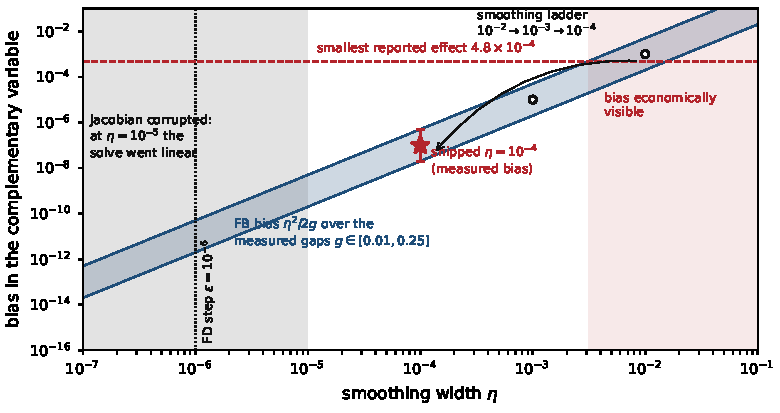
\includegraphics[width=0.70\textwidth]{fig_window.pdf}
\caption{\small The smoothing window. Left of $10^{-5}$ the Jacobian is corrupted (measured). Right
of about $3\times10^{-3}$ the bias reaches the size of reported effects. The shipped width and its
measured bias sit inside, and the smoothing ladder of \S\ref{sec:homotopy} walks in from the
visible region, where the switch is easy to follow but the answer is wrong, to the final width.}
\label{fig:window}
\end{figure}

\noindent The code actually uses \emph{two} smoothing widths, and the difference between them is
instructive. The guards (smooth floors and caps that keep the period map evaluable in extreme
states) use $10^{-5}$. They sit far from their bounds wherever the economy actually lives, so $g$ is
large and the bias at the rest point is about $10^{-11}$. The backstop's complementarity uses
$10^{-4}$. It sits \emph{on} its corner by design --- its floor binds at $43$ of the $115$ nodes ---
so it must be wide enough for the Jacobian to see through. Same formula, different $g$, different
answer.

\begin{lever}{the smoothing width $\eta$}
\leverrow{Controls}{How sharply a switch is resolved, and how far the smoothed model sits from the
true one.}
\leverrow{Push small}{The bias vanishes, but once $\eta$ approaches the finite-difference step the
Jacobian's relative error $\varepsilon/2\eta$ blows up: at $\eta=10\varepsilon$ Newton went linear.}
\leverrow{Push large}{The switch becomes a gentle ramp. Newton loves it, but the bias $\eta^2/g$
reaches the size of reported effects near $\eta\approx3\times10^{-3}$, and the solution is a solution
of a different model.}
\leverrow{Here}{$10^{-4}$ for the switch the economy sits on, reached by the ladder
$10^{-2}\to10^{-3}\to10^{-4}$; $10^{-5}$ for the guards it rarely approaches.}
\end{lever}

\paragraph{Smoothing protects the fit, too.} One more reason every guard is smooth. A \emph{hard}
clip on a value that is later \emph{fitted} puts a corner inside the box, and \S\ref{sec:1d} showed
what polynomials do with corners: one clipped node was measured to move the fitted rule at the
centre of the box by $26\%$, enough to drive it negative. And a hard floor is a flat plateau with
zero slope, so an iterate that lands on it is invisible to the finite-difference Jacobian and never
leaves (one such point sat at a residual of $4\times10^8$ indefinitely). The single hard $\max$
left in the solver is the one in \eqref{eq:muclosed}, and deliberately so: it is not a guard, it is
the economics.

\subsection{One smooth variable for two branches}
\label{sec:gz}

\begin{idea}
The backstop either buys bonds, in which case the price sits exactly at its floor, or does not, in
which case the price is free and above the floor. Both the purchase and the price have a corner at
the switch, and fitting either with a polynomial would invite the Gibbs overshoot. The trick is to
find a single variable that moves smoothly through the switch and describes both.
\end{idea}

\noindent The Garcia--Zangwill reformulation introduces one unknown $x$:
\begin{equation}
  \boxed{\;m = B\cdot\max(x,0),\qquad Q = Q^{\mathrm{floor}} + \bar Q\cdot\max(-x,0)\;}
  \label{eq:gz}
\end{equation}

\begin{reading}
$m$ is the purchase, $B$ the debt stock, $Q$ the bond price, $\bar Q$ its steady-state value.
When $x>0$, the central bank buys a share $x$ of the stock and the second $\max$ is zero, so the
price is at the floor. When $x<0$, nothing is bought and the price sits $-x\bar Q$ above the floor.
At most one $\max$ is ever nonzero, so the complementarity holds \emph{by construction}. And
although $m$ and $Q$ each have a corner at $x=0$, $x$ itself passes straight through zero: the rule
the solver stores and fits is smooth.
\end{reading}

\noindent What happens otherwise was measured. Storing the purchase directly, a coarse quadratic in
risk bought $19.7\%$ of the debt stock at a shock where the floor does not bind at all, and a
higher-degree fit turned the same corner into \emph{sales} between nodes. Fitting $x$ and recovering
$m$ and $Q$ pointwise removes both artefacts.

\paragraph{Root in one form, read in the other.} One final twist. The Garcia--Zangwill form is the
right one to \emph{store}, but Newton stalled using it while walking the policy cap down (its
steps were cut to $1/64$), whereas the Fischer--Burmeister form \eqref{eq:fb} took full steps. Since
both describe the same allocation at every node (measured: the Garcia--Zangwill residual evaluated
at the Fischer--Burmeister solution is $2.2\times10^{-9}$), the solver roots in one form, converts at
the nodes, and finishes with one or two Newton steps in the other. \emph{The formulation that is good
for the solver and the one that is good for the approximation need not be the same; when they agree
at the nodes, use both.}

\begin{incode}
\code{\_fb}, \code{\_smax} and \code{\_sclip} in \file{point\_map.py} are \eqref{eq:fb} and
\eqref{eq:smax}; \code{\_GUARD\_EPS} (the guards' width, $10^{-5}$) and \code{tpi\_eps} (the
backstop's width, $10^{-4}$, in the calibration) are the two widths. \code{\_incentive\_constraint}
is \eqref{eq:muclosed}; \code{\_tpi\_purchase\_and\_price} is \eqref{eq:gz}; \code{tpi\_gz} chooses
the form, and \code{\_tpi\_form} converts between them.
\end{incode}

\subsection{The corner is also an accuracy limit}

Everything above makes the corner \emph{solvable}. None of it makes the approximation \emph{exact}
at the corner, and in this model that limit is economically visible.

At the original calibration, the economy's long-run resting point sat exactly on the corner of
\eqref{eq:muclosed}: $\mu=0$, coverage exactly at the edge. By Figure \ref{fig:kink}(a), a polynomial
fitted through such a corner returns positive values where the truth is zero. So there are two ways
to read the solution at the same state, and they disagree:
\begin{itemize}
\item \textbf{read the fitted rule}, which prices a credit spread that is not really there, and
output falls;
\item \textbf{clear the equations exactly at that state}, which keeps $\mu=0$ until the default
probability reaches about $1.5\%$, and output barely moves.
\end{itemize}
At the headline shock the two gave output responses of $-0.081\%$ and $-0.008\%$: \emph{they disagreed
by more than the response itself.} More nodes helped only slowly (the gap fell from $0.087$ to $0.073$
percentage points going from $21$ to $95$ points), as the Gibbs analysis predicts.

\paragraph{What to do.} Three responses, all used here.

\emph{First, report both reads.} The honest object is the pair. This pathology is not peculiar to
this model: the same measurement on Bocola's published solution gives a fitted liquidity premium of
$28.4$ basis points where the exact multiplier gives $2.1$.

\emph{Second, move the economy off the corner.} The gap is largest when the constraint is exactly
marginal at rest. The steady-state credit-spread target controls how tightly the constraint binds,
and raising it lifts the resting multiplier off zero:

\begin{center}\small
\begin{tabular}{@{}rrrrrl@{}}
\toprule
spread target & resting $\mu$ & output, fitted & output, exact & gap (pp) & \\
\midrule
$8$ bp/yr   & $0.000$  & $-0.094\%$ & $-0.007\%$ & $0.087$ & on the corner\\
$25$ bp/yr  & $0.000$  & $-0.097\%$ & $-0.061\%$ & $0.036$ & \\
$100$ bp/yr & $0.0098$ & $-0.102\%$ & $-0.123\%$ & $\mathbf{0.021}$ & shipped\\
$250$ bp/yr & $0.0286$ & $-0.096\%$ & $-0.118\%$ & $0.022$ & no further gain\\
\bottomrule
\end{tabular}
\end{center}

\noindent The gap shrinks fourfold, and the fitted and exact reads now agree on the sign and the
order of magnitude. The obvious alternative lever, the bankers' exit rate $f$, does \emph{not} do
this: the calibration forces the franchise value to equal $\lambda$ times target leverage in the
steady state whatever $f$ is, so the binding margin is set by the spread, not by $f$. Finding the
lever that actually moves an approximation problem requires tracing the calibration, not guessing.

\emph{Third, state the limit.} Even at $100$ basis points, the \emph{level} of the output response is
bracketed rather than pinned down. The sign, the mechanism and the relative sizes are robust; the
second significant figure of the level is not. That is a legitimate result, provided it is reported.

\begin{lever}{the steady-state credit-spread target}
\leverrow{Controls}{How tightly the borrowing limit binds at rest, and so how far the resting economy
sits from the corner of $\mu$.}
\leverrow{Push small}{The economy rests on the corner. The fitted and exact reads of the solution
disagree by more than the response being measured (at $8$ bp: $0.087$ points against a $-0.094\%$
response).}
\leverrow{Push large}{The constraint binds firmly and the identification gap stays small, but beyond
$100$ bp nothing more is gained and the franchise value climbs steeply ($1.18$ at $100$ bp, $1.61$ at
$250$, $15.8$ at $650$). Above $672$ bp the bank calibration has no solution at all; both
boundaries are derived in closed form in \S\ref{sec:reference}.}
\leverrow{Here}{$100$ bp per year: where the constraint starts to bind at rest, Gertler and
Kiyotaki's own target, and within the $100$--$300$ bp range of euro-periphery lending spreads in
2011--12.}
\end{lever}

%======================================================================
\section{Expectations over a continuous shock and a discrete event}
\label{sec:quad}

\begin{idea}
Every Euler equation contains an expectation: an integral over tomorrow's shock. The computer cannot
integrate exactly, so it replaces the integral by a weighted average over a few well-chosen values of
the shock. The art is choosing the values and weights so that a handful of them integrate a smooth
function almost exactly.
\end{idea}

\subsection{Gauss--Hermite quadrature}

The risk factor's innovation is a standard normal $\varepsilon$. The rule replaces
\begin{equation}
  \E\big[h(\varepsilon)\big] = \int h(\varepsilon)\,\frac{e^{-\varepsilon^2/2}}{\sqrt{2\pi}}\,d\varepsilon
  \qquad\text{by}\qquad
  \sum_{q=1}^{n} w_q\,h(\varepsilon_q).
\end{equation}

\begin{reading}
With $n$ nodes you choose $2n$ numbers: $n$ locations and $n$ weights. That is enough to match $2n$
conditions, so you can demand that the rule be exact for $h(\varepsilon) = 1,\varepsilon,\dots,
\varepsilon^{2n-1}$ --- every polynomial of degree up to $2n-1$. Gaussian quadrature is the choice
that achieves this. A rule with fixed, equally spaced nodes has only $n$ free weights and can match
only degree $n-1$: half as good, for the same work.
\end{reading}

\noindent The solver uses $n=5$, exact to degree $9$. You can watch the boundary on the shipped rule:
it gives $\E[\varepsilon^8]=105$, which is exact, and $\E[\varepsilon^{10}] = 825$, where the truth is
$945$. Past degree $2n-1$, the guarantee stops.

\subsection{A convention trap worth a whole paragraph}

Two versions of Hermite quadrature are in common use, and they differ by a factor of $\sqrt2$:
\begin{itemize}
\item the \emph{probabilists'} rule integrates against $e^{-x^2/2}$, so its nodes
($0,\pm1.356,\pm2.857$ for $n=5$) are already in standard deviations, and
$s' = \text{mean} + \sigma_s\varepsilon_q$ is correct;
\item the \emph{physicists'} rule integrates against $e^{-x^2}$, and its nodes ($0,\pm0.959,\pm2.020$)
are the probabilists' divided by exactly $\sqrt2$.
\end{itemize}
Use physicists' nodes in $s' = \text{mean}+\sigma_s\varepsilon_q$, forgetting the $\sqrt2$, and you have
quietly integrated against a normal with standard deviation $\sigma_s/\sqrt2$. Bocola's code does
precisely this, so his reported innovation of $0.63$ behaves inside his solved model as
$0.63/\sqrt2 = 0.4455$. Importing the reported $0.63$ into a correct probabilists' rule reproduces his
\emph{parameter} but not his \emph{model}: the unconditional standard deviation of $s$ becomes $2.02$
instead of $1.43$, and the long-run average default probability $0.66\%$ per quarter instead of
$0.27\%$. The solver uses the probabilists' rule with $\sigma_s=0.4455$. \emph{When replicating a
paper, check its quadrature convention before concluding anything about its parameters.}

\subsection{Mixing in the default event}

The default indicator $d'$ is discrete: tomorrow is in the default world with probability
$p^d(s)$ and in the no-default world otherwise, and each world has its own rule. The expectation is
a sum over cells, one for each pair of innovation node and world:
\begin{equation}
  \E[h] \;=\; \sum_{q=1}^{n}\;\sum_{d'\in\{0,1\}}\;
  \underbrace{w_q\,\Big[d'\,p^d(s) + (1-d')\big(1-p^d(s)\big)\Big]}_{\text{probability of the cell}}
  \;h\big(\varepsilon_q,d'\big).
  \label{eq:product}
\end{equation}
The two cells in each column add up to $w_q$, so the measure is preserved exactly.

\begin{reading}
The term $h(\varepsilon_q,1)$ is not a stylised ``default penalty''. It is the \emph{same solved
rules}, for the default world, evaluated at the state the economy would actually reach. That matters
because the banker's marginal value of wealth $\Omega$ is high in that world, where its bonds have just
lost $55\%$. So the bond pays least exactly when wealth is worth most, and \eqref{eq:product} prices
that covariance as a risk premium. An earlier version of the model priced default with a single
representative branch instead, and got the \emph{sign} of the whole mechanism wrong: sovereign risk
came out expansionary.
\end{reading}

\noindent Two properties are worth engineering in deliberately. First, when $p^d=0$ the default
world carries no weight; the code then skips it entirely, so switching risk off reproduces the
risk-free model \emph{bit for bit}, not merely to a tolerance. That is a far sharper regression test.
Second, the quadrature order is recorded with the solution and reused by everything that later reads
it. A rule solved at $n=5$ and read back at $n=7$ is a slightly different object, and the difference
would be charged to whatever economic question is being asked.

\begin{lever}{the quadrature order $n$}
\leverrow{Controls}{How accurately each expectation is computed: exact to degree $2n-1$.}
\leverrow{Push to 1}{The innovation is replaced by its mean: the solution sees no risk in $s$ at all,
only the discrete default event.}
\leverrow{Push up}{Expectations converge quickly for smooth integrands, but every node is another full
evaluation of tomorrow's economy in both worlds, so cost rises in proportion.}
\leverrow{Here}{$5$, exact to degree $9$. Whatever order is used to solve must also be used to read.}
\end{lever}

\begin{incode}
\code{gh\_nodes} in \file{point\_map.py} uses NumPy's \code{hermegauss}, the probabilists' rule.
\code{\_regime\_weights} builds the cell probabilities of \eqref{eq:product}, \code{\_expect} sums them,
and \code{\_continuation} skips a zero-weight world. The order is \code{N\_GH} (the quadrature node
count) in \file{recursive\_experiment.py}, stamped on the solution as \code{RuleSet.n\_gh}.
\end{incode}

%======================================================================
\part*{Part IV \quad Reading the answer}
\addcontentsline{toc}{section}{\textbf{Part IV\quad Reading the answer}}
%======================================================================
\section{Where does the economy actually live?}
\label{sec:reading}

\begin{idea}
A solved rule is not yet an answer. To report an impulse response you must start the economy
somewhere and compare a shocked path with something. The natural choices --- start at the steady
state, compare with the steady state --- are both wrong in a model that prices risk, and the error
they introduce can be larger than the response itself.
\end{idea}

\subsection{The deterministic steady state is not the resting point}

The steady state is computed for an economy with no risk at all, and it is exact: solved with the
default probability set identically to zero, the model sits on it for two hundred quarters to six
decimal places. But the rules we solved for \emph{price risk}, and a risk-pricing economy does not
come to rest where its risk-free counterpart does. Three forces move it.

\begin{enumerate}
\item \textbf{Convexity.} The default probability is a convex function of $s$ over the relevant range,
so by Jensen's inequality its long-run \emph{average} exceeds its value at the average $s$: $0.27\%$
against $0.10\%$ per quarter, nearly three times as large.
\item \textbf{Premia.} Banks are paid a premium for holding risky bonds. On average they collect it,
so at rest they hold more net worth than in the risk-free steady state.
\item \textbf{The constraint.} More net worth means more coverage in \eqref{eq:muclosed}, a smaller
multiplier, and a lower credit spread.
\end{enumerate}

\noindent The current run measures the combined effect. Evaluating the solved rules at the
steady-state state vector and at the resting point gives:

\begin{center}\small
\begin{tabular}{@{}lrrr@{}}
\toprule
 & at the steady-state state & at the resting point & change \\
\midrule
multiplier $\mu_D$ & $0.0173$ & $0.0110$ & $-36\%$ \\
credit spread, bp/yr & $136.8$ & $88.7$ & $-48$ bp \\
bank net worth & & & $+2.05\%$ \\
banks' holdings of $D$ bonds & & & $+2.3\%$ \\
\bottomrule
\end{tabular}
\end{center}

\noindent This resting point is sometimes called the \emph{risky steady state}: the point where the
economy stays if no shock ever hits, \emph{while agents still expect that one might}. It is distinct
from the deterministic steady state (no risk, no shocks) and from the ergodic mean (risk, and shocks
actually hitting). It is also robust: it does not move with grid resolution, and eight deliberately
perturbed starting points all converge to it, to within $10^{-12}$.

\subsection{Finding it, and differencing twice}

The resting point is found the obvious way: start somewhere, apply the solved rule with every shock
set to zero, and repeat,
\begin{equation}
  \st_{t+1} = H\big(\st_t,\;\hat g(\st_t),\;\varepsilon_{t+1}=0\big),
  \qquad\text{until}\qquad \|\st_{t+1}-\st_t\| < 10^{-11}.
\end{equation}
Then every impulse response is computed in two steps:
\begin{enumerate}
\item it \textbf{starts} at the resting point, so deviations are measured from the level the economy
actually occupies; \emph{and}
\item it is \textbf{differenced} against an unshocked path from the same start,
\begin{equation}
  \hat y_t \;=\; \frac{y_t^{\text{shocked}}}{y_t^{\text{unshocked}}} - 1,
  \label{eq:diff}
\end{equation}
so that any drift common to both paths --- including drift caused by approximation error --- cancels.
\end{enumerate}

\noindent Skipping this is not a small error. In an earlier calibration, starting at the
deterministic steady state and comparing against it charged the economy's walk toward its resting
point to the shock: between $54\%$ and $63\%$ of a reported post-impact hump in output, and of a
reported $+4.2\%$ overshoot in bank net worth, turned out to be that walk. An apparent slow erosion of
the capital stock was almost entirely drift. A response computed that way reports a transition
between two resting points as if it were a response to a shock.

\subsection{Read the rule; do not re-solve it}

At any state you can either read the fitted rule's values, or re-solve the period's equations there
starting from them. They differ, and the first is the right default: \S\ref{sec:newton} showed that
re-solving near a switching constraint can slip onto the wrong branch and flip the sign of the
response. The re-solve is still useful in exactly one place, the deliberate \emph{pair} of reads at
the corner (\S\ref{sec:kink}), where the gap between them is itself the reported uncertainty.

\begin{lever}{the resting-point tolerance}
\leverrow{Controls}{How completely the no-shock simulation is allowed to settle before an impulse
response starts.}
\leverrow{Push loose}{The response starts part-way along the walk to rest. Differencing
\eqref{eq:diff} still removes the walk from the response, but deviations are then taken from a level
the economy does not occupy.}
\leverrow{Push tight}{More quarters of simulation; harmless, because each is one cheap read of the
rule.}
\leverrow{Here}{$10^{-11}$, with a warning printed if the walk has not settled to $10^{-8}$.}
\end{lever}

\begin{incode}
\code{stochastic\_rest\_point} in \file{recursive\_experiment.py} runs the no-shock simulation;
\code{dynamic\_irf} differences against the unshocked path; \code{read\_at} reads the rule and
\code{read\_exact} re-solves at a state. \code{report\_rest\_point} prints the table above.
\end{incode}

%======================================================================
\section{Is the answer right?}
\label{sec:accuracy}

\begin{idea}
A Newton residual of $10^{-9}$ is a statement about the collocation nodes, and only about them. It
says nothing about the error \emph{between} nodes, which is where the economy spends nearly all of its
time. Four independent checks answer the question that matters.
\end{idea}

\subsection{Euler errors where the economy lives}

Simulate the solved rule forward for $1200$ quarters with randomly drawn shocks. At every state
visited, evaluate all $20$ equilibrium conditions using the rule's own values, without re-solving,
and record each residual in $\log_{10}$ units. The units are interpretable. The household's Euler
residual is a relative error in the consumption composite, so $-4$ means the household's choice is off
by about one part in ten thousand: a precise economic statement, not an abstract tolerance.

The current run gives a mean of $-4.34$ over the $19$ economic equations. The weakest equation is the
franchise-value identity of the $D$ bank, whose worst case is $-2.33$; that is the same slowly-moving
object that defeated time iteration in \S\ref{sec:paradigms}, showing up again as the hardest thing to
represent. The best is the deposit-clearing condition, at $-6.24$.

\paragraph{A trap in the summary line.} The solver's printed table reports an overall mean of
$-4.92$, not $-4.34$. The difference is the backstop's residual, which with the backstop switched off
is identically zero and therefore enters as $\log_{10}$ of the smallest representable number, $-16$.
One equation that is trivially satisfied, averaged into twenty, makes the solution look about four
times more accurate than it is. \emph{When you average accuracy across equations, exclude the ones
that hold by construction.}

\subsection{Box escapes: the empirical answer to \S\ref{sec:box}}

The simulated path is recorded \emph{before} any projection back into the box, and the share of
quarters spent outside is reported for each state. This is the measured counterpart of the invariance
theory of \S\ref{sec:box}, which said that no axis-aligned box can be one-step invariant here. In
practice, across $1200$ quarters, the economy left the box in no state, not once (worst overshoot
$0.00\%$ of the box width). The theory gives the worst case over every point of the box; the
simulation shows that the economy never comes near the corners where the worst case happens. Both
facts are worth knowing, and only the second can be measured.

\subsection{A convergence study, in the units of the question}

The only direct evidence that a solution is resolved is to refine it and see what moves. Raising the
dense factor in $s$ from $5$ to $9$:

\begin{center}\small
\begin{tabular}{@{}lrrr@{}}
\toprule
 & 5 nodes (115 points) & 9 nodes (207 points) & move \\
\midrule
impact output response, fitted read & $-0.1105\%$ & $-0.1087\%$ & $1.6\%$ of itself \\
impact output response, exact read & $-0.1278\%$ & $-0.1234\%$ & $3.4\%$ of itself \\
credit spread response & $+90.6$ bp/yr & $+90.8$ bp/yr & third digit \\
$D$ bond price response & $-9.263\%$ & $-9.304\%$ & third digit \\
\bottomrule
\end{tabular}
\end{center}

\noindent Both output moves are far inside the gap between the fitted and exact reads
(\S\ref{sec:kink}). So the binding limit on this solution is the corner, not the resolution, and the
study says which lever to pull next: the calibration, not the grid. That is the useful output of a
convergence study --- not a reassurance, but a direction. It is also conditional. Before the
recalibration of \S\ref{sec:kink}, refinement was fighting a Gibbs phenomenon and more nodes bought
little; a convergence study has to be re-run after any change of calibration.

\subsection{Redundant equations as free checks}

By Walras's law one market-clearing condition follows from all the others plus the budget
constraints. The solver \emph{drops} the $F$ goods market and the current account from the system ---
including them would make the Jacobian singular --- and \emph{monitors} them instead. They are an
independent audit: an error in any budget constraint anywhere in the model shows up there, and no
amount of Newton convergence on the retained equations can hide it. In this model the check earned
its keep: it exposed a constant household transfer standing in for a working-capital flow that the
retained system was perfectly content with. \emph{Identify the redundancies, drop them from the solve,
and watch them.}

\begin{lever}{the length of the accuracy simulation}
\leverrow{Controls}{How well the reported errors describe the economy's long-run distribution.}
\leverrow{Push short}{The mean is noisy and the maximum, a tail statistic, is badly underestimated:
rare excursions toward the corners of the box are never visited.}
\leverrow{Push long}{Cost grows linearly, one cheap read per quarter; the risk is only of averaging
away a localised problem, which is why the table reports the maximum and the 90th percentile as well
as the mean.}
\leverrow{Here}{$1200$ quarters after a $200$-quarter burn-in.}
\end{lever}

\begin{incode}
\file{accuracy.py}: \code{simulate} draws the path without clipping it, \code{euler\_errors}
evaluates the residuals at the rule's own values, and \code{accuracy\_report} prints the per-equation
table and the box escapes. The length is \code{ACCURACY\_T} (simulated quarters) in \file{run.py}.
\end{incode}

%======================================================================
\part*{Part V \quad Reference}
\addcontentsline{toc}{section}{\textbf{Part V\quad Reference}}
%======================================================================
\section{The bank calibration's limits, and the guards}
\label{sec:reference}

\subsection{Two boundaries in closed form}

The steady state pins the bank's frictions from two targets, leverage $\theta$ and the credit spread
$s$ (quarterly). Combining the binding constraint with the franchise recursion \eqref{eq:franchise}
gives the steady-state multiplier directly:
\begin{equation}
  \bar\mu \;=\; \frac{s\,\theta}{1+r+s\,\theta}.
  \label{eq:muss}
\end{equation}
At the calibration ($s = 100$ bp/yr, $\theta=5$, $r=0.003$) this is $0.0123$, matching the solver to
eight decimals. Two things can go wrong as $s$ rises.

\paragraph{The entrant transfer turns negative.} New bankers receive a transfer
$\omega = D/\theta - (1-f)s$, with $D = 1-(1-f)(1+r) = f(1+r) - r$. It must be positive, which requires
\begin{equation}
  s \;<\; \frac{f(1+r)-r}{(1-f)\,\theta} \;\approx\; 672\ \text{bp per year}.
\end{equation}

\paragraph{The franchise recursion folds.} By \eqref{eq:slope} the recursion turns explosive when
$\bar\mu$ exceeds $1-\beta(1-f)R \approx f$. Setting \eqref{eq:muss} equal to $f$ and solving,
\begin{equation}
  s \;=\; \frac{f(1+r)}{(1-f)\,\theta} \;\approx\; 698\ \text{bp per year}.
\end{equation}
The two boundaries differ only by the deposit-rate term $r/((1-f)\theta)$, which is $26$ bp. The code
agrees with both: at $650$ bp it solves (with a franchise value already exploding to $15.8$, against
$1.18$ at the shipped $100$ bp), at $690$ bp it reports a negative entrant transfer, and from $700$ bp
on it finds no root at all.

\paragraph{Picking the right root.} Below the fold the franchise equation generally has \emph{two}
roots, a stable low one and an unstable high one. Iterating the recursion from below converges to the
low root, so the calibration must select the same one or the model and its calibration describe
different economies. The code therefore does not hand the equation to a root-finder with a starting
guess, which could land on either. It scans for sign changes on a logarithmic grid from $10^{-6}$ to
$10^{6}$, brackets the \emph{first} crossing, and only then refines. A scan cannot pick the wrong
root; a Newton step can.

\subsection{Guards}

Every parameter below exists only to keep the period map evaluable at extreme states, because an
error inside a single finite-difference column ruins the entire Jacobian. Each one is smoothed, each
is inactive where the economy lives, and each is exposed so its effect can be measured rather than
trusted.

\begin{center}\small
\begin{tabular}{@{}>{\raggedright\arraybackslash}p{0.30\textwidth}>{\raggedright\arraybackslash}p{0.20\textwidth}>{\raggedright\arraybackslash}p{0.43\textwidth}@{}}
\toprule
Guard & Value & Prevents \\
\midrule
cap on the franchise value $\alpha$ & $40$ & divergence beyond the fold, in deep default states \\
cap on the multiplier $\mu$ & $0.95$ & $\alpha=\E[\Omega]R/(1-\mu)$ blowing up as $\mu\to1$ \\
floor on bank net worth & $0.15\times$ steady state & insolvent banks in the deepest default corners \\
floor on next-period capital & feasibility $\times1.0001$ & an investment rate the adjustment cost cannot produce \\
bounds on consumption & $[0.15,\,3]\times$ steady state & negative or absurd consumption in a trial step \\
floor on the GHH composite & $5\%$ of steady-state $C$ & a zero-gradient plateau in the discount factor \\
\bottomrule
\end{tabular}
\end{center}

\noindent The net-worth floor deserves a note: unlike the others, it is switched on for every
production run (\code{NW\_FLOOR}, the floor as a share of steady-state net worth, in \file{run.py}). It
never binds on the ergodic set, but the default-regime solve depends on it, so it is part of the
solved model.

\section{Every lever at both extremes}

\begin{center}\small
\begin{longtable}{@{}>{\raggedright\arraybackslash}p{0.17\textwidth}>{\raggedright\arraybackslash}p{0.25\textwidth}>{\raggedright\arraybackslash}p{0.25\textwidth}>{\raggedright\arraybackslash}p{0.24\textwidth}@{}}
\toprule
\textbf{Lever} & \textbf{Too small} & \textbf{Too large} & \textbf{Here, and why} \\
\midrule
\endfirsthead
\toprule
\textbf{Lever} & \textbf{Too small} & \textbf{Too large} & \textbf{Here, and why} \\
\midrule
\endhead
\multicolumn{4}{@{}l}{\emph{Representing the rule}}\\[2pt]
nodes per dimension $m$ & no response to the state & cost; kinks barely improve & level 2, plus a dense factor in $s$ \\
Smolyak budget $\mu$ & every state looks the same & cost grows like $d^{\mu}$ & $1$: no cross terms between ordinary states \\
dense factor $m_s$ & $3$: shock mispriced by $2/3$, negative probabilities & cost $\propto n^2$ & $5$; confirmed at $9$ \\
box coverage $\kappa$ & clipping changes the dynamics & resolution wasted, unsolvable corners & $2.75$ s.d.; no escapes \\
\addlinespace
\multicolumn{4}{@{}l}{\emph{Solving}}\\[2pt]
damping $\omega$ & nothing moves & overshoot near switches & $0.5$, warm start only \\
finite-difference step $\varepsilon$ & noise $2\delta/\varepsilon$ dominates & slope error $\varepsilon/2\eta$ on kinks & $10^{-6}$ \\
acceptance on $\max|F|$ & below the floor: stalls & solver error looks like economics & $10^{-9}$ \\
Jacobian reuse & (fresh each step) & convergence turns linear & every step \\
homotopy step & many costly rungs & start outside the basin & fixed rungs; halve on failure \\
warm-start sweeps & seed outside the basin & wasted sweeps & $12$; $20$ on refined grids \\
\addlinespace
\multicolumn{4}{@{}l}{\emph{Nonsmoothness and expectations}}\\[2pt]
smoothing $\eta$ & Jacobian corrupted & bias $\eta^2/g$ visible & $10^{-4}$ (switch), $10^{-5}$ (guards) \\
spread target & economy rests on the corner & franchise value explodes; no root above $672$ bp & $100$ bp/yr \\
quadrature order $n$ & risk in $s$ invisible & cost $\propto n$ & $5$, exact to degree $9$ \\
\addlinespace
\multicolumn{4}{@{}l}{\emph{Reading}}\\[2pt]
rest-point tolerance & response starts mid-walk & harmless & $10^{-11}$ \\
accuracy length & tails unseen & cost $\propto T$ & $1200$ quarters \\
\bottomrule
\end{longtable}
\end{center}

\section{The whole algorithm on one page}

\begin{framed}\small
\noindent\textbf{1. Steady state.} Solve the bank's franchise equation for its least root (sign scan,
then refine); recover the frictions from the leverage and spread targets. Solve for the returns and
the terms of trade that clear capital markets and external balance, rescale productivity so output is
one, then solve the household discount factors that clear deposits. Calibrate the household transfer
so the steady state is an exact rest point.

\smallskip\noindent\textbf{2. Grid.} Build the box (bands around the steady state, $\kappa$ standard
deviations in $s$, the shear for the policy book). Build the sparse grid at budget $\mu=1$ over eleven
states, tensored with $m_s$ dense nodes in $s$; factor $\Phi$ once.

\smallskip\noindent\textbf{3. Cold start.} Every rule at its steady-state value, except next period's
capital, which follows the state's own capital so investment is feasible at every node.

\smallskip\noindent\textbf{4. The ladder} (each rung: a short time-iteration warm start, then Newton).
No-default regime at zero risk $\to$ default regime by haircut ($0.85\to0.45$) $\to$ both regimes
jointly with risk priced $\to$ (if the backstop is on) its cap from $700$ bp down, halving failed
rungs $\to$ the dense factor in $s$ raised, with the smoothing walked in on each refined grid.

\smallskip\noindent\textbf{5. Inside one evaluation of $F$.} Fit the coefficients to the current node
values. At every node and regime: production, the fiscal block, balance sheets, then the expectation
over (innovation node $\times$ world) using the current fitted rule; discount factors; the closed-form
multiplier; bond demands; wages; households; stack $14$ residuals and append the $6$ identity
residuals. A node that cannot be evaluated returns a large sentinel, so one bad point costs the step,
not the solve.

\smallskip\noindent\textbf{6. Newton.} Finite-difference Jacobian on every core; LU factor; line search
on $\tfrac12\|F\|^2$; stop at $\max|F|\le10^{-9}$, or at the arithmetic floor ($\le10^{-8}$) when no
step helps.

\smallskip\noindent\textbf{7. Read.} Find the resting point by no-shock simulation; compute every
response from it, differenced against the unshocked path; report the fitted and exact reads as a pair.

\smallskip\noindent\textbf{8. Check.} Euler errors on a $1200$-quarter simulation, excluding equations
that hold by construction; box escapes; the Walras-redundant markets; a convergence run at higher
resolution.
\end{framed}

\section{Where each idea lives in the code}

\noindent Files are in \file{global\_projection/solver\_recursive/} unless another directory is given.

\begin{center}\small
\begin{longtable}{@{}>{\raggedright\arraybackslash}p{0.27\textwidth}>{\raggedright\arraybackslash}p{0.68\textwidth}@{}}
\toprule
\textbf{File} & \textbf{Ideas from this document} \\
\midrule
\endfirsthead
\toprule
\textbf{File} & \textbf{Ideas from this document} \\
\midrule
\endhead
\file{state\_grid.py} & Chebyshev polynomials and nodes, the Smolyak budget, new points and
degrees, the dense factor, the box and its coverage, rotation and shear
(\S\ref{sec:1d}--\ref{sec:box}) \\
\file{decision\_rules.py} & the $20$ stored rules, fitting in logs and gross rates, the two regimes \\
\file{point\_map.py} & one evaluation of the economy at a node: the closed-form multiplier,
Fischer--Burmeister, smooth guards, Garcia--Zangwill, the expectation over shocks and worlds
(\S\ref{sec:kink}--\ref{sec:quad}) \\
\file{collocation.py} & the global residual $F$, identity residuals, Newton, the finite-difference
Jacobian on every core, Newton--Krylov (\S\ref{sec:paradigms}--\ref{sec:newton}) \\
\file{recursive\_main.py} & time iteration as a warm start; measuring $J$ for the rotation \\
\file{recursive\_experiment.py} & the ladder (\S\ref{sec:homotopy}); the resting point, differencing,
and the pair of reads (\S\ref{sec:reading}) \\
\file{accuracy.py} & Euler errors and box escapes (\S\ref{sec:accuracy}) \\
\file{blocks/bank.py} {\footnotesize(one level up)} & the franchise equation, its least root, the two
boundaries (\S\ref{sec:reference}) \\
\file{run.py} {\footnotesize(repo root)} & resolution, accuracy length, the net-worth floor, which
experiments run \\
\file{calibration/} {\footnotesize(repo root)} & every economic parameter, and the backstop's
smoothing \\
\bottomrule
\end{longtable}
\end{center}

\section{Further reading}

\noindent\emph{Approximation.} L.\ N.\ Trefethen, \emph{Approximation Theory and Approximation
Practice} (SIAM, 2013): the clearest modern account of everything in \S\ref{sec:1d}, including the
Lebesgue constant and the Bernstein-ellipse theorem. S.\ A.\ Smolyak (1963) for the original sparse
grid; V.\ Barthelmann, E.\ Novak and K.\ Ritter, ``High dimensional polynomial interpolation on sparse
grids'', \emph{Advances in Computational Mathematics} (2000), for its error theory.

\noindent\emph{Projection methods in economics.} K.\ L.\ Judd, ``Projection methods for solving
aggregate growth models'', \emph{Journal of Economic Theory} (1992), where it starts; and his
\emph{Numerical Methods in Economics} (MIT Press, 1998). D.\ Krueger and F.\ Kubler (2004) and B.\
Malin, D.\ Krueger and F.\ Kubler (2011), both in the \emph{Journal of Economic Dynamics and Control},
for Smolyak collocation in economics; K.\ Judd, L.\ Maliar, S.\ Maliar and R.\ Valero (2014), same
journal, for anisotropic grids. J.\ Fern\'andez-Villaverde, J.\ Rubio-Ram\'irez and F.\ Schorfheide,
``Solution and estimation methods for DSGE models'', \emph{Handbook of Macroeconomics} (2016), for the
landscape.

\noindent\emph{Newton, continuation, complementarity.} C.\ T.\ Kelley, \emph{Iterative Methods for
Linear and Nonlinear Equations} (SIAM, 1995): line searches, chord methods, and why Krylov methods need
preconditioning. E.\ Allgower and K.\ Georg, \emph{Numerical Continuation Methods} (Springer, 1990),
for \S\ref{sec:homotopy}. F.\ Facchinei and J.-S.\ Pang, \emph{Finite-Dimensional Variational Inequalities
and Complementarity Problems} (Springer, 2003), for Fischer--Burmeister; C.\ B.\ Garcia and W.\ I.\
Zangwill, \emph{Pathways to Solutions, Fixed Points, and Equilibria} (Prentice-Hall, 1981), for
\S\ref{sec:gz}.

\noindent\emph{Accuracy and reading.} M.\ S.\ Santos, ``Accuracy of numerical solutions using the Euler
equation residuals'', \emph{Econometrica} (2000). N.\ Coeurdacier, H.\ Rey and P.\ Winant, ``The risky
steady state'', \emph{American Economic Review Papers \& Proceedings} (2011), for \S\ref{sec:reading}.

\noindent\emph{The economics.} L.\ Bocola, ``The pass-through of sovereign risk'', \emph{Journal of
Political Economy} (2016), whose solution design this solver follows; M.\ Gertler and P.\ Karadi (2011)
and M.\ Gertler and N.\ Kiyotaki (2010) for the bank and its borrowing limit.

\end{document}
